\documentclass[10pt,twocolumn,letterpaper]{article}

\usepackage{cvpr}
\usepackage{times}
\usepackage{epsfig}
\usepackage{graphicx}
\usepackage{amsmath}
\usepackage{amssymb}

\usepackage{subcaption}
\usepackage{multirow}
\usepackage{graphicx}
\usepackage{subcaption}

% Include other packages here, before hyperref.

% If you comment hyperref and then uncomment it, you should delete
% egpaper.aux before re-running latex.  (Or just hit 'q' on the first latex
% run, let it finish, and you should be clear).
\usepackage[breaklinks=true,bookmarks=false]{hyperref}

\def\cvprPaperID{****} % *** Enter the CVPR Paper ID here
\def\httilde{\mbox{\tt\raisebox{-.5ex}{\symbol{126}}}}

% Pages are numbered in submission mode, and unnumbered in camera-ready
%\ifcvprfinal\pagestyle{empty}\fi
\setcounter{page}{1}
\begin{document}
\pagestyle{plain}

%%%%%%%%% TITLE
\title{MLCV Coursework 1 Report}

\author{Shinyoung Yu\\
20200405\\
School of Computing\\
{\tt\small sahaa0918@kaist.ac.kr}
% For a paper whose authors are all at the same institution,
% omit the following lines up until the closing ``}''.
% Additional authors and addresses can be added with ``\and'',
% just like the second author.
% To save space, use either the email address or home page, not both
\and
Jiyun Park\\
20210263\\
School of Computing\\
{\tt\small jiyun02@kaist.ac.kr}
}

\maketitle
%\thispagestyle{empty}

% \begin{abstract}
The ABSTRACT is to be in fully justified italicized text, at the top of the left-hand column, below the author and affiliation information.
Use the word ``Abstract'' as the title, in 12-point Times, boldface type, centered relative to the column, initially capitalized.
The abstract is to be in 10-point, single-spaced type.
Leave two blank lines after the Abstract, then begin the main text.
Look at previous \confName abstracts to get a feel for style and length.
\end{abstract}   
\section{Eigenfaces}
\label{sec:intro}

Face data is the base dataset for our experiment. This consists of 520 data with 52 classes and 10 data for each class. We will conduct the upcoming experiments by dividing the data for each class into an 8:2 train-test split.

%-------------------------------------------------------------------------
\subsection{Eigenfaces}

There are two method to conduct PCA: PCA($S=AA^T$) and low dimensional PCA($S=A^TA$). We compare two methods on training dataset with size 2576*416(D*N).

\begin{figure}[htbp]
	\centering
	\begin{subfigure}[t]{0.48\linewidth}
		\centering
		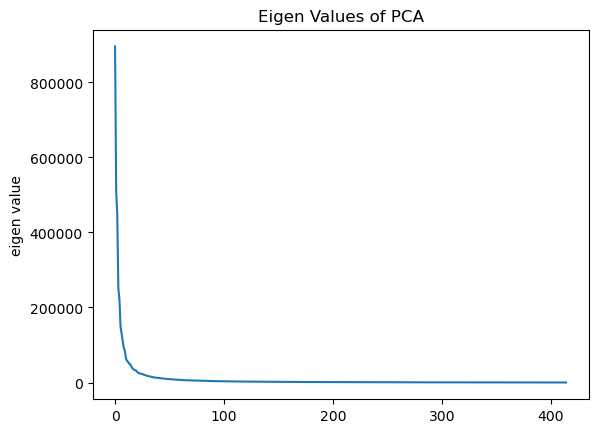
\includegraphics[width=\linewidth]{image/q1_eigval_pca.png}
		\caption{nonzero eigenvalues of PCA}
		\label{fig:eigval_pca}
	\end{subfigure}%
	\hfill
	\begin{subfigure}[t]{0.48\linewidth}
		\centering
		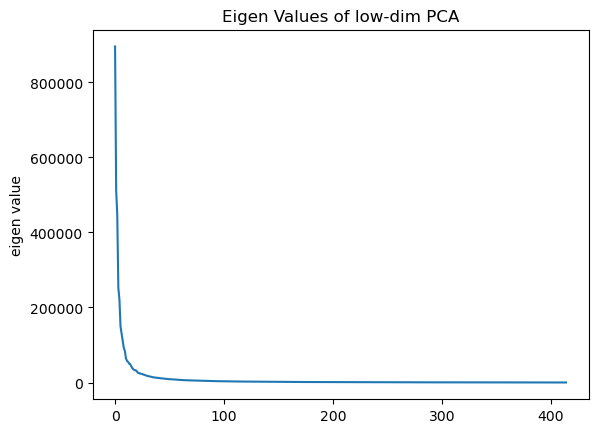
\includegraphics[width=\linewidth]{image/q1_eigval_lowdim.png}
		\caption{nonzero eigenvalues of low-dimensional PCA}
		\label{fig:eigval_lowdim}
	\end{subfigure}
	\caption{Comparison between eigenvalues of PCA methods}
	\label{fig:q1_eigval}
\end{figure}

As shown in \cref{fig:q1_eigval} both methods have the same nonzero eigenvalues. Specifically, PCA has 2576 nonzero eigenvalues, and low-dimensional PCA has 416. However, when selecting values bigger than $\frac{1}{100}$, both methods yield 415 eigenvalues. This is because, given matrix sizes of 2576x2576 and 416x416, the maximum ranks are 2576 and 416, respectively. But since we have 416 data points, the PCA projection subspace can at most capture 415 meaningful dimensions, resulting in 415 eigenvalues larger than $\frac{1}{100}$. From this comparison (\cref{fig:q1_eigval}), we conclude that both methods yield the same eigenvalues, and their top 415 eigenvectors are also identical.

The only difference between them is computation time: PCA takes 8.015s, while low-dimensional PCA takes 1.092s. Low-dimensional PCA is faster because, in our case, the data dimension exceeds the number of data points, making its covariance matrix smaller than that of PCA. Based on this time efficiency, we use low-dimensional PCA going forward. % 시간복잡도는 O(N^3)인데 이것보단 적게 차이나는데 어쩌지!!


\subsection{Image reconstuction using Eigenfaces}
Using pca basis from above, we perform face reconstruction. \cref{fig:recon_train} and \cref{fig:recon_test} shows reconstruction results using different numbers of PCA bases. As seen in the images, the reconstruction become more accurate with more bases. When using only 10 bases, the results resemble the mean face(\cref{fig:q1_meanface}) of training data. This occurs because the PCA basis is oriented to capture common features by maximizing data variance. Thus, with a small number of bases, the reconstruction reflects common features of the dataset more strongly than specific details of each image.

\begin{figure}
	\centering
	\begin{subfigure}[t]{0.2\linewidth}
		\centering
		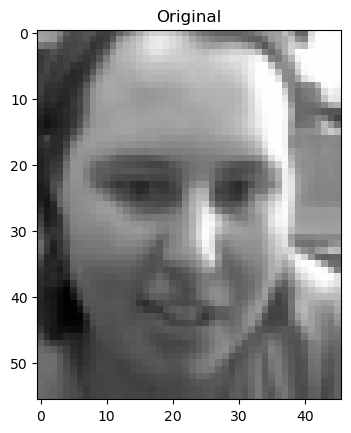
\includegraphics[width=\linewidth]{image/q1_recon_train_original.png}
		\caption{original}
		\label{fig:train_re_original}
	\end{subfigure}%
	\hfill
	\begin{subfigure}[t]{0.2\linewidth}
		\centering
		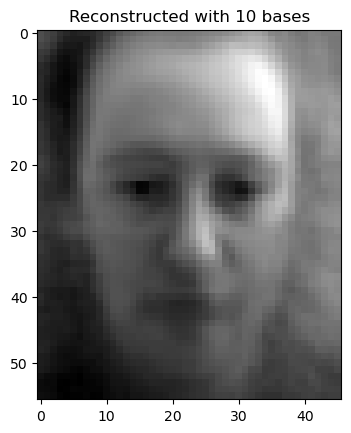
\includegraphics[width=\linewidth]{image/q1_recon_train_10.png}
		\caption{10 bases}
		\label{fig:train_re_10}
	\end{subfigure}
    \hfill
	\begin{subfigure}[t]{0.2\linewidth}
		\centering
		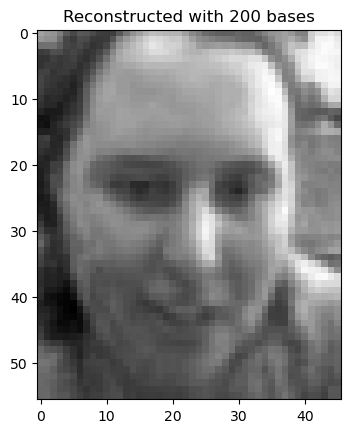
\includegraphics[width=\linewidth]{image/q1_recon_train_200.png}
		\caption{200 bases}
		\label{fig:train_re_200}
	\end{subfigure}
    \hfill
	\begin{subfigure}[t]{0.2\linewidth}
		\centering
		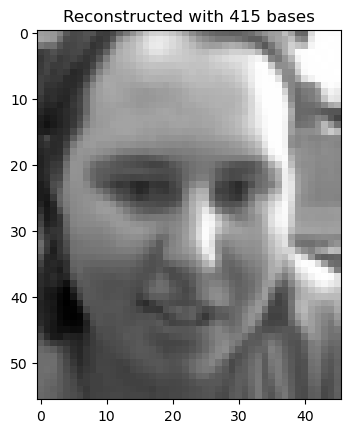
\includegraphics[width=\linewidth]{image/q1_recon_train_415.png}
		\caption{415 bases}
		\label{fig:train_re_415}
	\end{subfigure}
	\caption{Training data reconstruction results}
	\label{fig:recon_train}
\end{figure}

\begin{figure}
	\centering
	\begin{subfigure}[t]{0.2\linewidth}
		\centering
		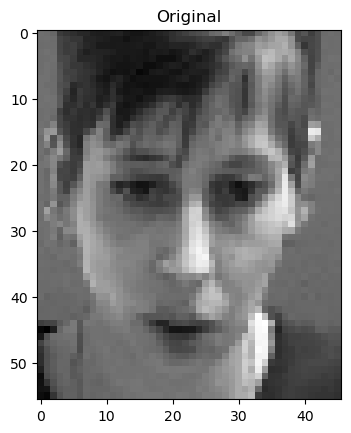
\includegraphics[width=\linewidth]{image/q1_recon_test_original.png}
		\caption{original}
		\label{fig:test_re_original}
	\end{subfigure}%
	\hfill
	\begin{subfigure}[t]{0.2\linewidth}
		\centering
		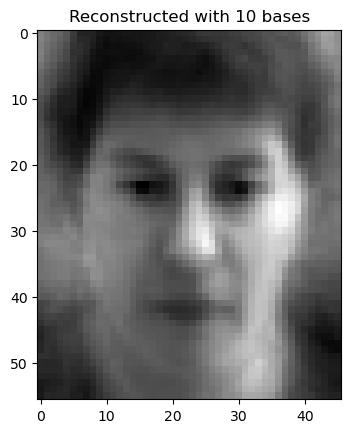
\includegraphics[width=\linewidth]{image/q1_recon_test_10.png}
		\caption{10 bases}
		\label{fig:test_re_10}
	\end{subfigure}
    \hfill
	\begin{subfigure}[t]{0.2\linewidth}
		\centering
		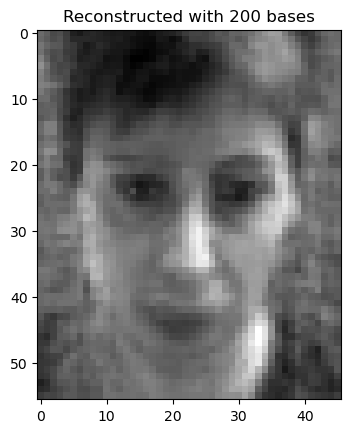
\includegraphics[width=\linewidth]{image/q1_recon_test_200.png}
		\caption{200 bases}
		\label{fig:test_re_200}
	\end{subfigure}
    \hfill
	\begin{subfigure}[t]{0.2\linewidth}
		\centering
		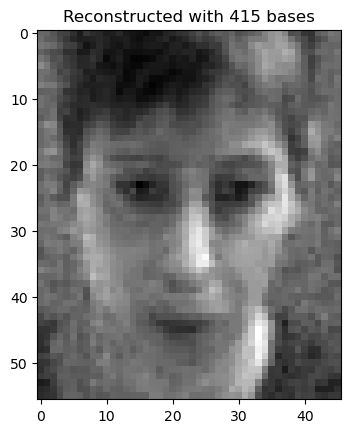
\includegraphics[width=\linewidth]{image/q1_recon_test_415.png}
		\caption{415 bases}
		\label{fig:test_re_415}
	\end{subfigure}
	\caption{Test data reconstruction results}
	\label{fig:recon_test}
\end{figure}

For more detailed analysis, we computed the reconstruction error. The theoretical error is given by $\sum_{i=n+1}^M \lambda_i$ where $n$is the number of bases we used for the reconstruction, $M$is total number of PCA bases, and $\lambda_i$ is eigenvalues of unused eigenvectors. The actual reconstruction error can be calculated using L2-norm of difference between the original and reconstructed data.

\begin{figure}
	\centering
	\begin{subfigure}[t]{0.48\linewidth}
		\centering
		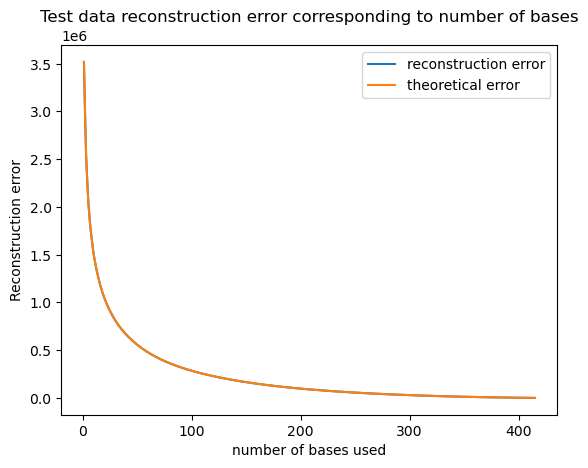
\includegraphics[width=\linewidth]{image/q1_recon_error_train.png}
		\caption{training data}
		\label{fig:recon_error_train}
	\end{subfigure}%
	\hfill
	\begin{subfigure}[t]{0.48\linewidth}
		\centering
		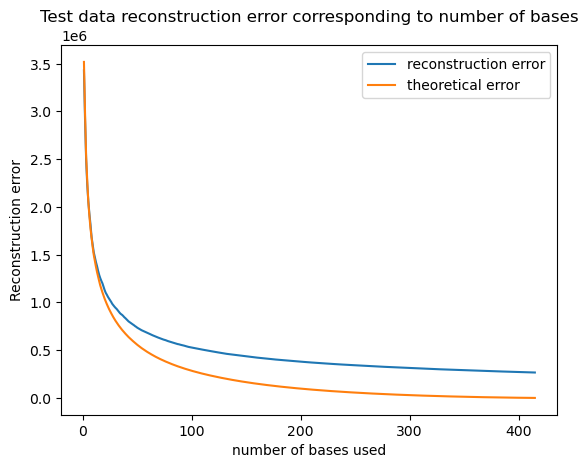
\includegraphics[width=\linewidth]{image/q1_recon_error_test.png}
		\caption{test data}
		\label{fig:recon_error_test}
	\end{subfigure}
	\caption{PCA reconstruction error}
	\label{fig:recon_error}
\end{figure}

As shown in \cref{fig:recon_error}, the reconstruction error from the training data matched the theoretical result. However, for the test data, while the graph’s shape was similar to the theoretical result, the actual values differed slightly. This may be because the PCA bases used for reconstruction were derived from the training data, not the test data.

\subsection{KNN classification using Eigenfaces}

We can also perform classification using PCA with NN classifier. As shown in \cref{fig:q1_knn_accuracy}, accuracy improves with more PCA bases and fewer neighbors($k$). More PCA bases preserve more data information, leading to accurate projections in the PCA subspace. For the number of neighbors, using fewer makes the classifier more sensitive to local information and better at preserving class boundaries, thus increasing classification accuracy.

In terms of time and memory, the number of neighbors made no significant difference. However, as shown in \cref{fig:q1_knn_time} and \cref{fig:q1_knn_memory}, the execution time and memory usage of the k-NN classifier linearly increase  with the number of PCA bases increase. This is because, the execution time and memory usage is $O(N\cdot M)$ where $N$ is the number of total data and $M$ is the number of PCA bases we used. Since $k$ only affects on final selection process, its impact during the computation is very small.

\begin{figure}
	\centering
	
	% 윗줄에 하나의 이미지, 크기는 0.48로 유지
	\begin{subfigure}[t]{0.48\linewidth}
		\centering
		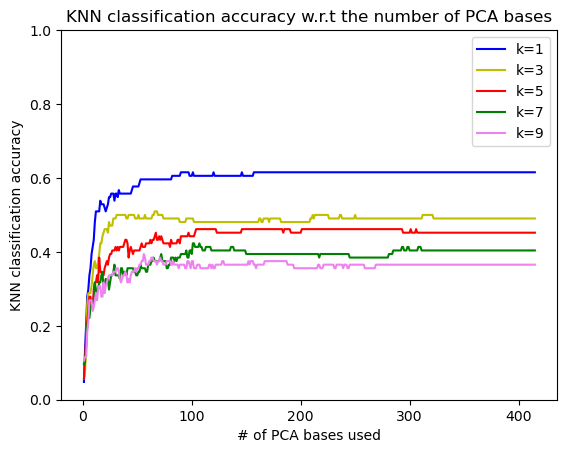
\includegraphics[width=\linewidth]{image/q1_accuracy.png}
		\caption{accuracy}
		\label{fig:q1_knn_accuracy}
	\end{subfigure}
	
    \vspace{0.5cm} % 이미지들 사이에 공간 추가

	% 아랫줄에 두 개의 이미지, 크기 동일하게 0.48
	\begin{subfigure}[t]{0.48\linewidth}
		\centering
		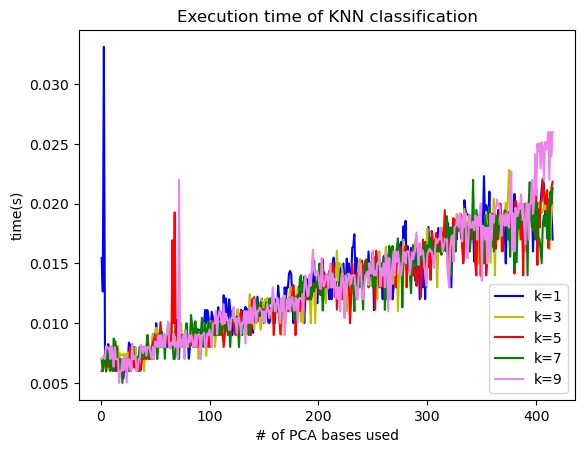
\includegraphics[width=\linewidth]{image/q1_time.png}
		\caption{running time}
		\label{fig:q1_knn_time}
	\end{subfigure}%
	\hfill
	\begin{subfigure}[t]{0.48\linewidth}
		\centering
		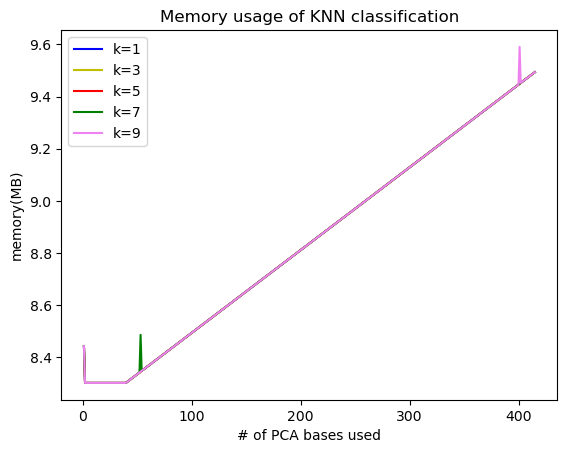
\includegraphics[width=\linewidth]{image/q1_memory.png}
		\caption{memory usage}
		\label{fig:q1_knn_memory}
	\end{subfigure}

	\caption{Analysis on KNN classification using PCA}
	\label{fig:pca_knn}
\end{figure}

However, its overall prediction accyracy is about 0.6, which is not that high. This might because, PCA is not very sophisticated model to capture all the detailed features of data. As we also check from the confusion matrix(\cref{fig:q1_cm}), there are many components outside the diagonal, that failed to be predicted.


Detailed prediction examples can be found in Appendix B, C.
\section{Incremental PCA}
\label{sec:intro}

%-------------------------------------------------------------------------
\subsection{Important parameter in implementation: $d_3$}
To implement incremental PCA, we utilized the algorithm from the "Online Learning" slides presented in class. Here, a key parameter is $d_2$ and $d_3$. When new data arrives in incremental PCA, computing the eigenspace model for this subset requires $O(\min(D, N')^3)$ time, where $N'$ is the number of data points in the subset. Additionally, merging this new eigenspace model with the existing data takes $O((d_1 + d_2 + 1)^3)$ time, where $d_1$ is equal to the previously computed eigenspace model's $d_3$ value. Therefore, to enhance time efficiency in incremental PCA, it is essential to keep $d_3$ small, although this results in a time-accuracy tradeoff by dropping less-significant eigenvector information, which is represented by our experiment result \cref{fig:q2-fig5}
\vspace{-0.5cm}

\begin{figure}[htbp]
	\centering
	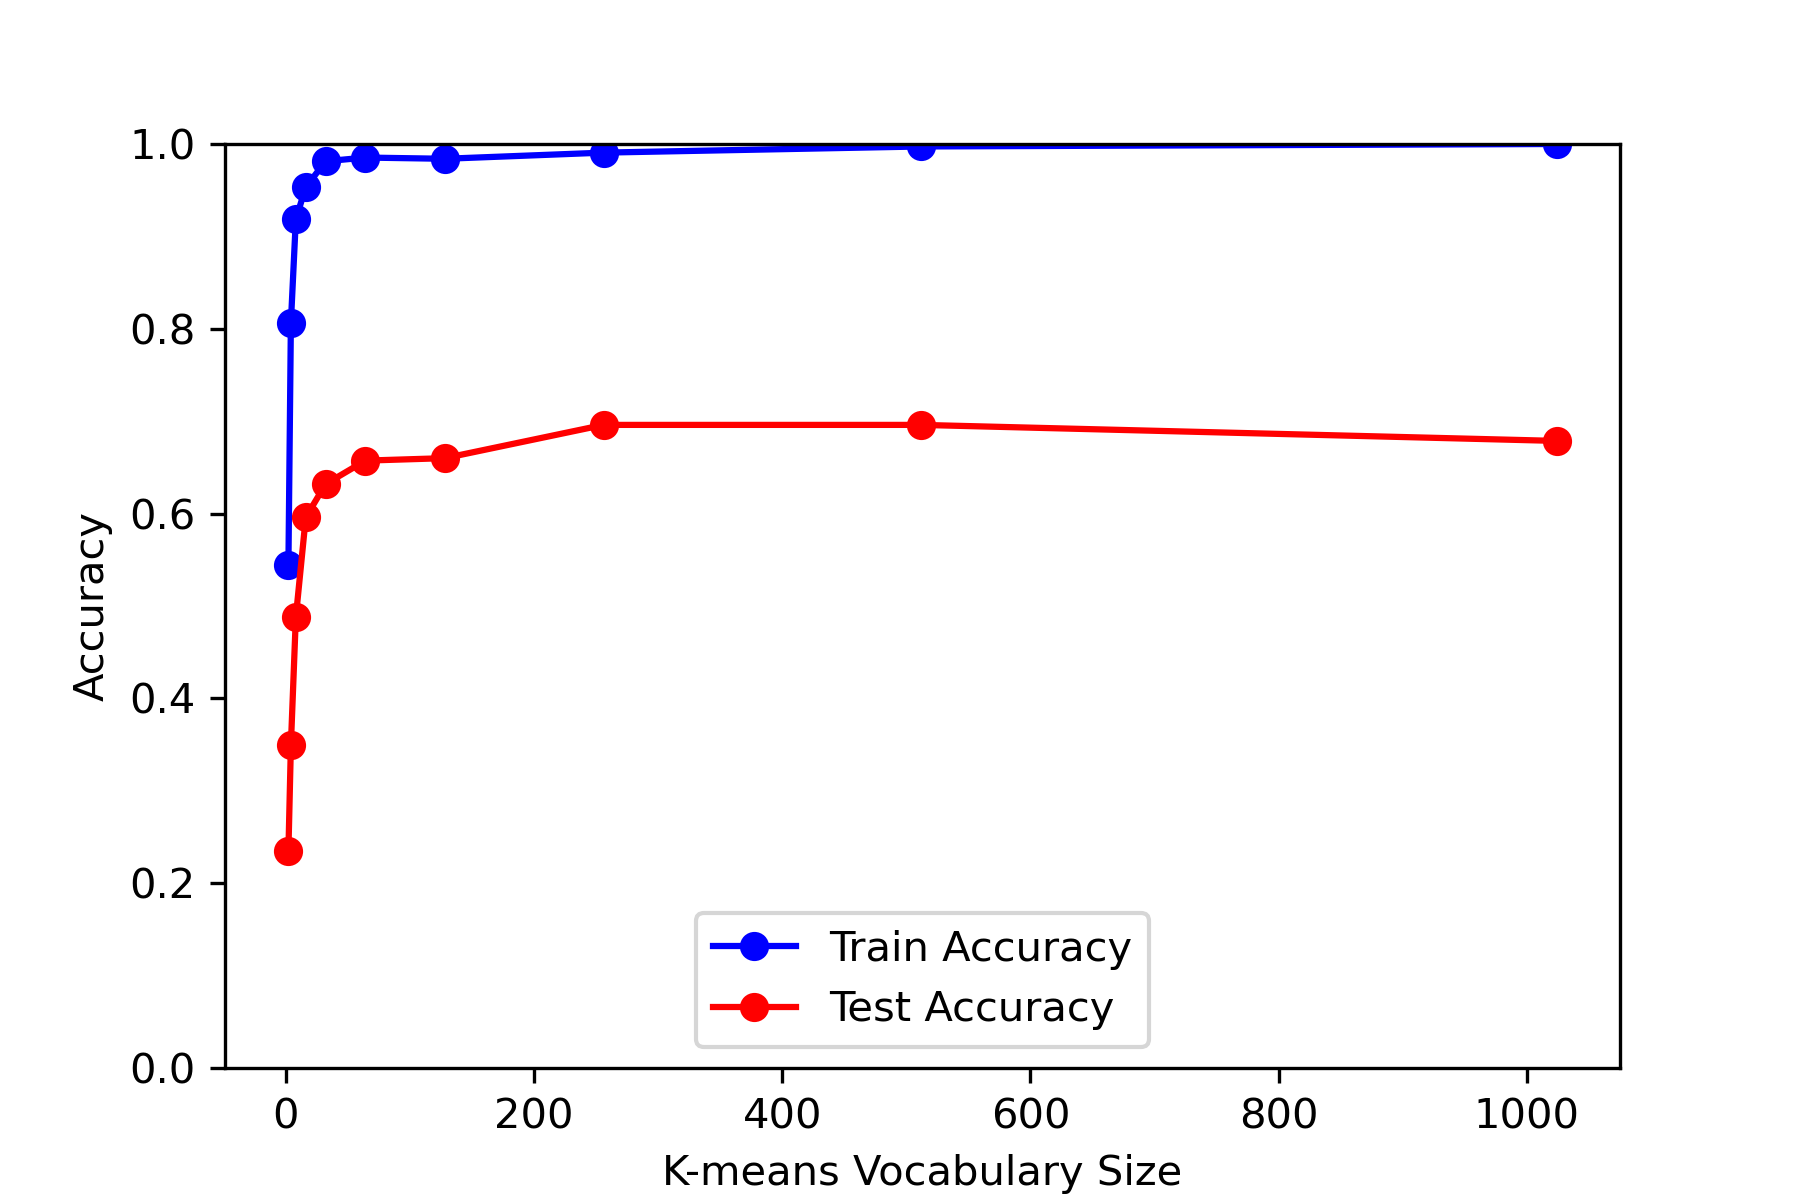
\includegraphics[width=\linewidth]{image/q2-fig5.png}
	
	\caption{Incremental PCA's time-accuracy tradeoff according to the value of $d_3$}
	\label{fig:q2-fig5}
\end{figure}
\vspace{-0.5cm}

\subsection{Comparison with other PCA}
We compared the results of each incremental PCA stage (i.e.adding training data in four batches) with the results of batch PCA in the following four aspects. In summary, incremental PCA is a good approximation of batch PCA, and even requires less training time.
\begin{itemize}
	\item Training time: For batch PCA, we measured training time by re-training the model each time new data was added. The results are shown in \cref{fig:q2-fig1}. Using one subset, the training time is approximately the same for both methods. However, as we add more data, the value of $N$ increases for batch PCA, while the values of $N'$ and $d_3$ remain constant for incremental PCA, maintaining constant time and improving time-wise efficiency.
	
	\item Accuracy of incremental PCA: In incremental PCA, time-accuracy tradeoff occurs since less-significant eigenvectors are dropped during $d_1 + d_2$ merging, retaining only the top $d_3$ eigenvectors. We calculated the cosine similarity of eigenvectors, eigenvalues, and mean vectors between incremental PCA at each stage and batch PCA calculated by corresponding data, as shown in \cref{fig:q2-fig2}. As more training data is added, the number of discarded less-significant eigenvectors increases, resulting in decreased similarity between eigenvectors; the similarity after adding the last subset is 0.856. For mean vectors and eigenvalues, cosine similarities are 1 and close to 1 respectively, indicating that the incremental PCA is a good approximation.
	
	\item Reconstruction error: Referring to \cref{fig:q2-fig3}, the reconstruction error for incremental PCA using all training data (i.e., after adding the 4th batch) is almost identical to that of batch PCA with the same amount of data. This also demonstrates that incremental PCA gives similar result to batch PCA.
	
	\item Face recognition accuracy: In the optimal settings of batch PCA found in Question1 (i.e. K=1 and bases=90) the accuracy ranks as follows: full-data batch PCA $>$ full-data incremental PCA $>$ PCA using only the first training set. This indicates that classification accuracy improves progressively with the increase in training data. Additionally, using incremental PCA in place of batch PCA results in an accuracy drop of approximately 6.67\%, also indicating a time-accuracy tradeoff.
	
\end{itemize}

\vspace{-0.5cm}
\begin{figure}[htbp]
	\centering
	\begin{subfigure}{0.48\linewidth}
		\centering
		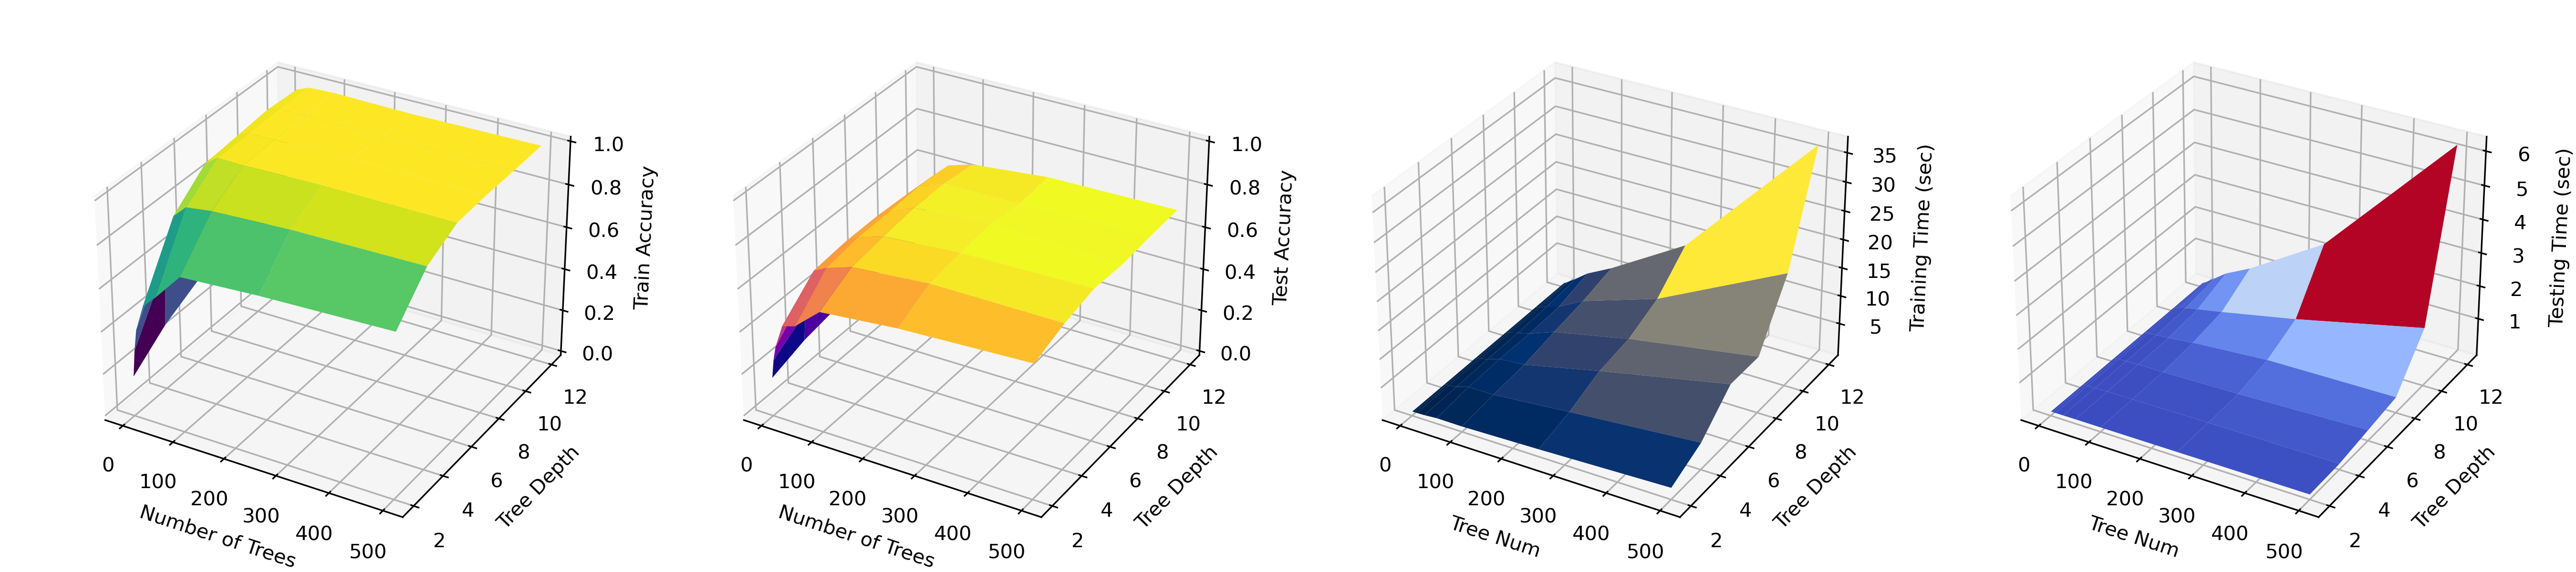
\includegraphics[width=\linewidth]{image/q2-fig1.png}
		\caption{Training time}
		\label{fig:q2-fig1}
	\end{subfigure}%
	\hfill
	\begin{subfigure}{0.48\linewidth}
		\centering
		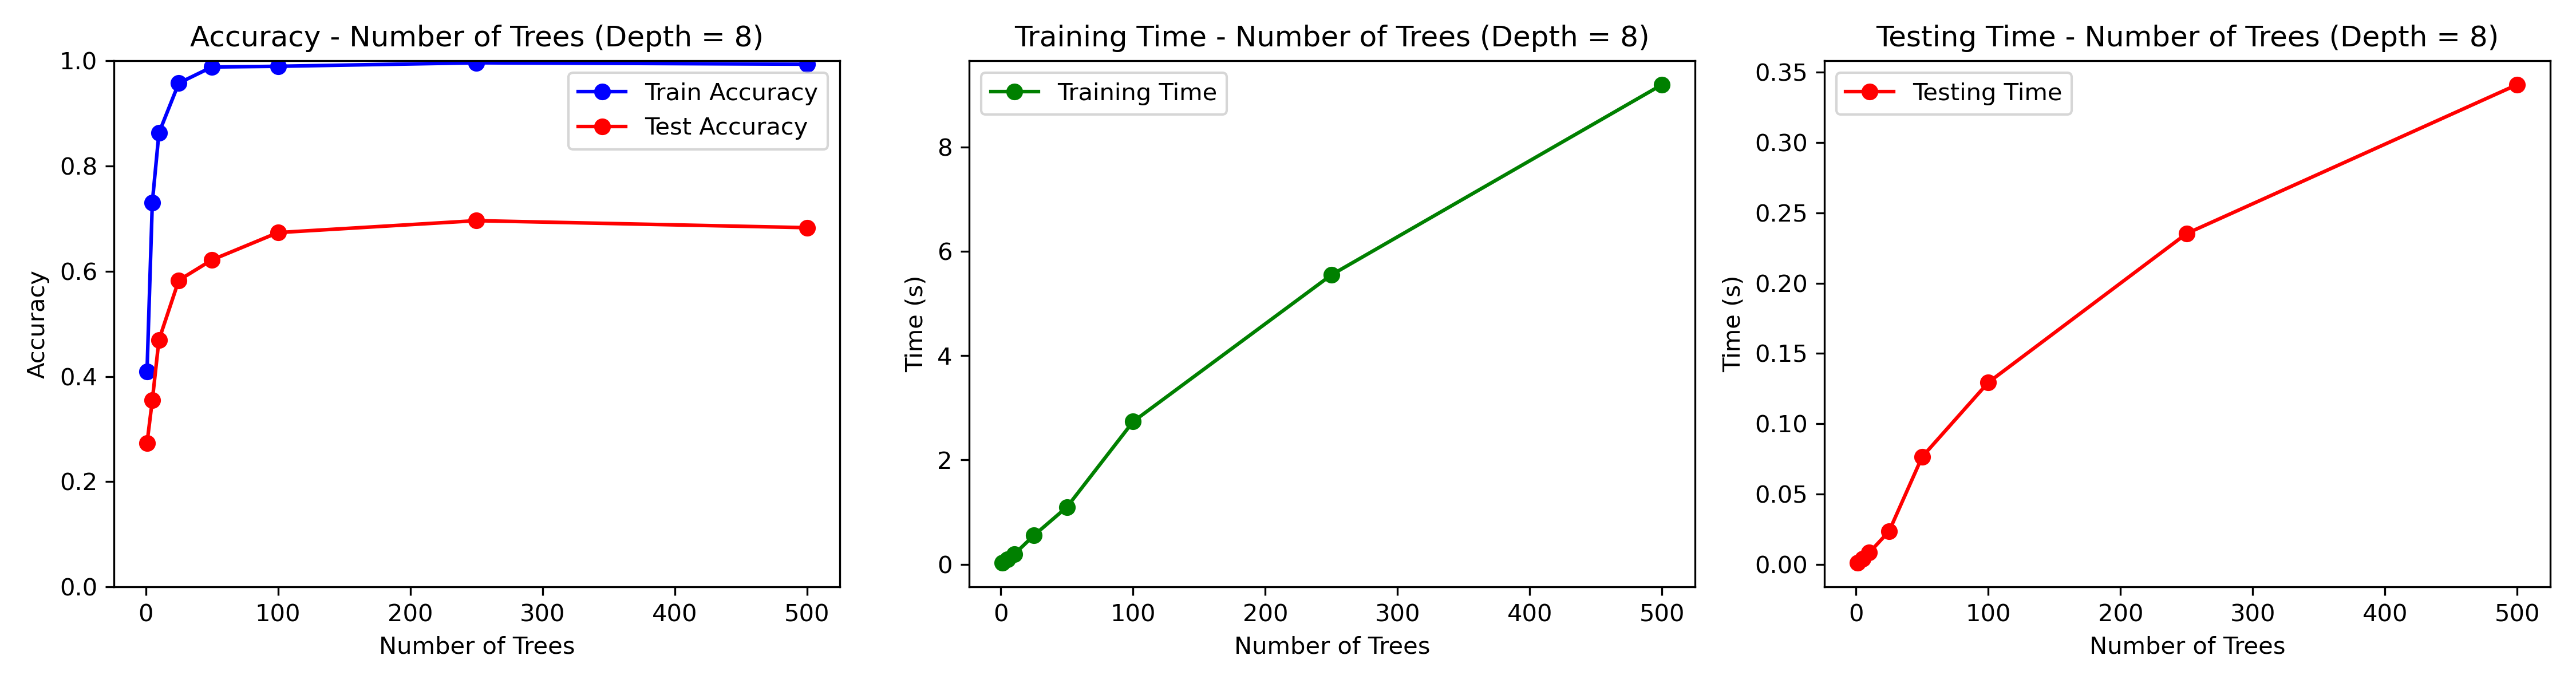
\includegraphics[width=\linewidth]{image/q2-fig2.png}
		\caption{Cosine similarity of results}
		\label{fig:q2-fig2}
	\end{subfigure}
	
	\begin{subfigure}{0.48\linewidth}
		\centering
		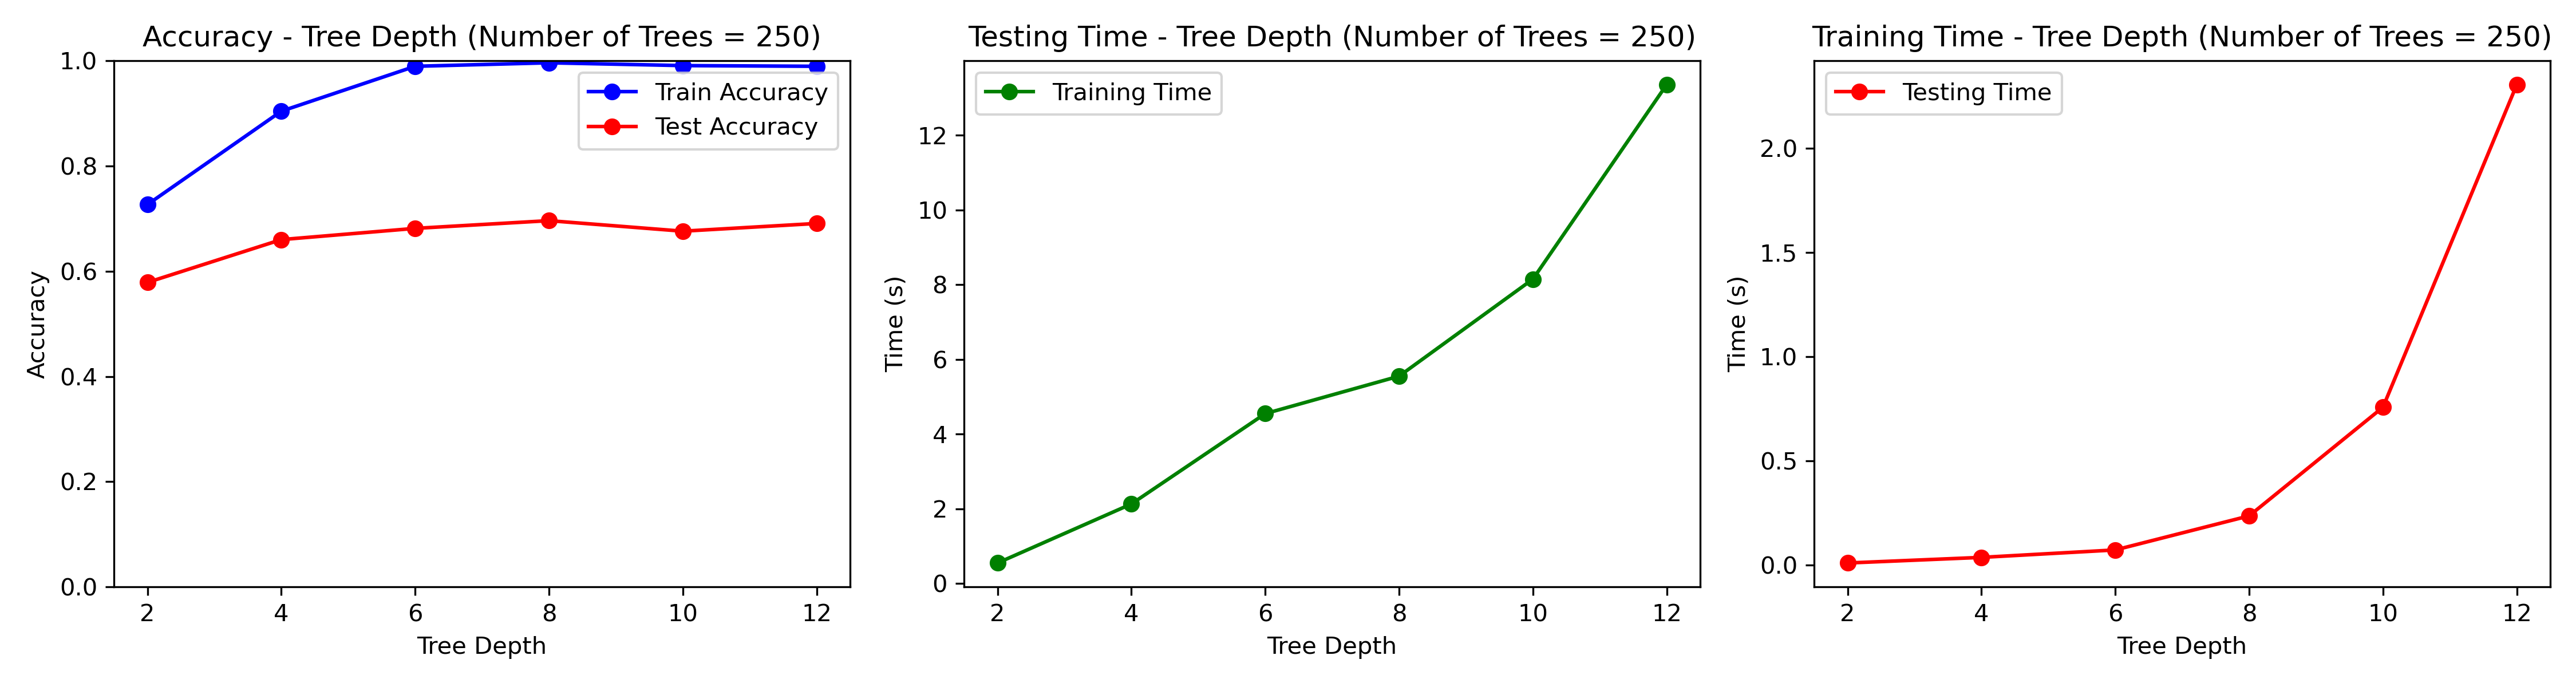
\includegraphics[width=\linewidth]{image/q2-fig3.png}
		\caption{Reconstruction error}
		\label{fig:q2-fig3}
	\end{subfigure}
	\hfill
	\begin{subfigure}{0.48\linewidth}
		\centering
		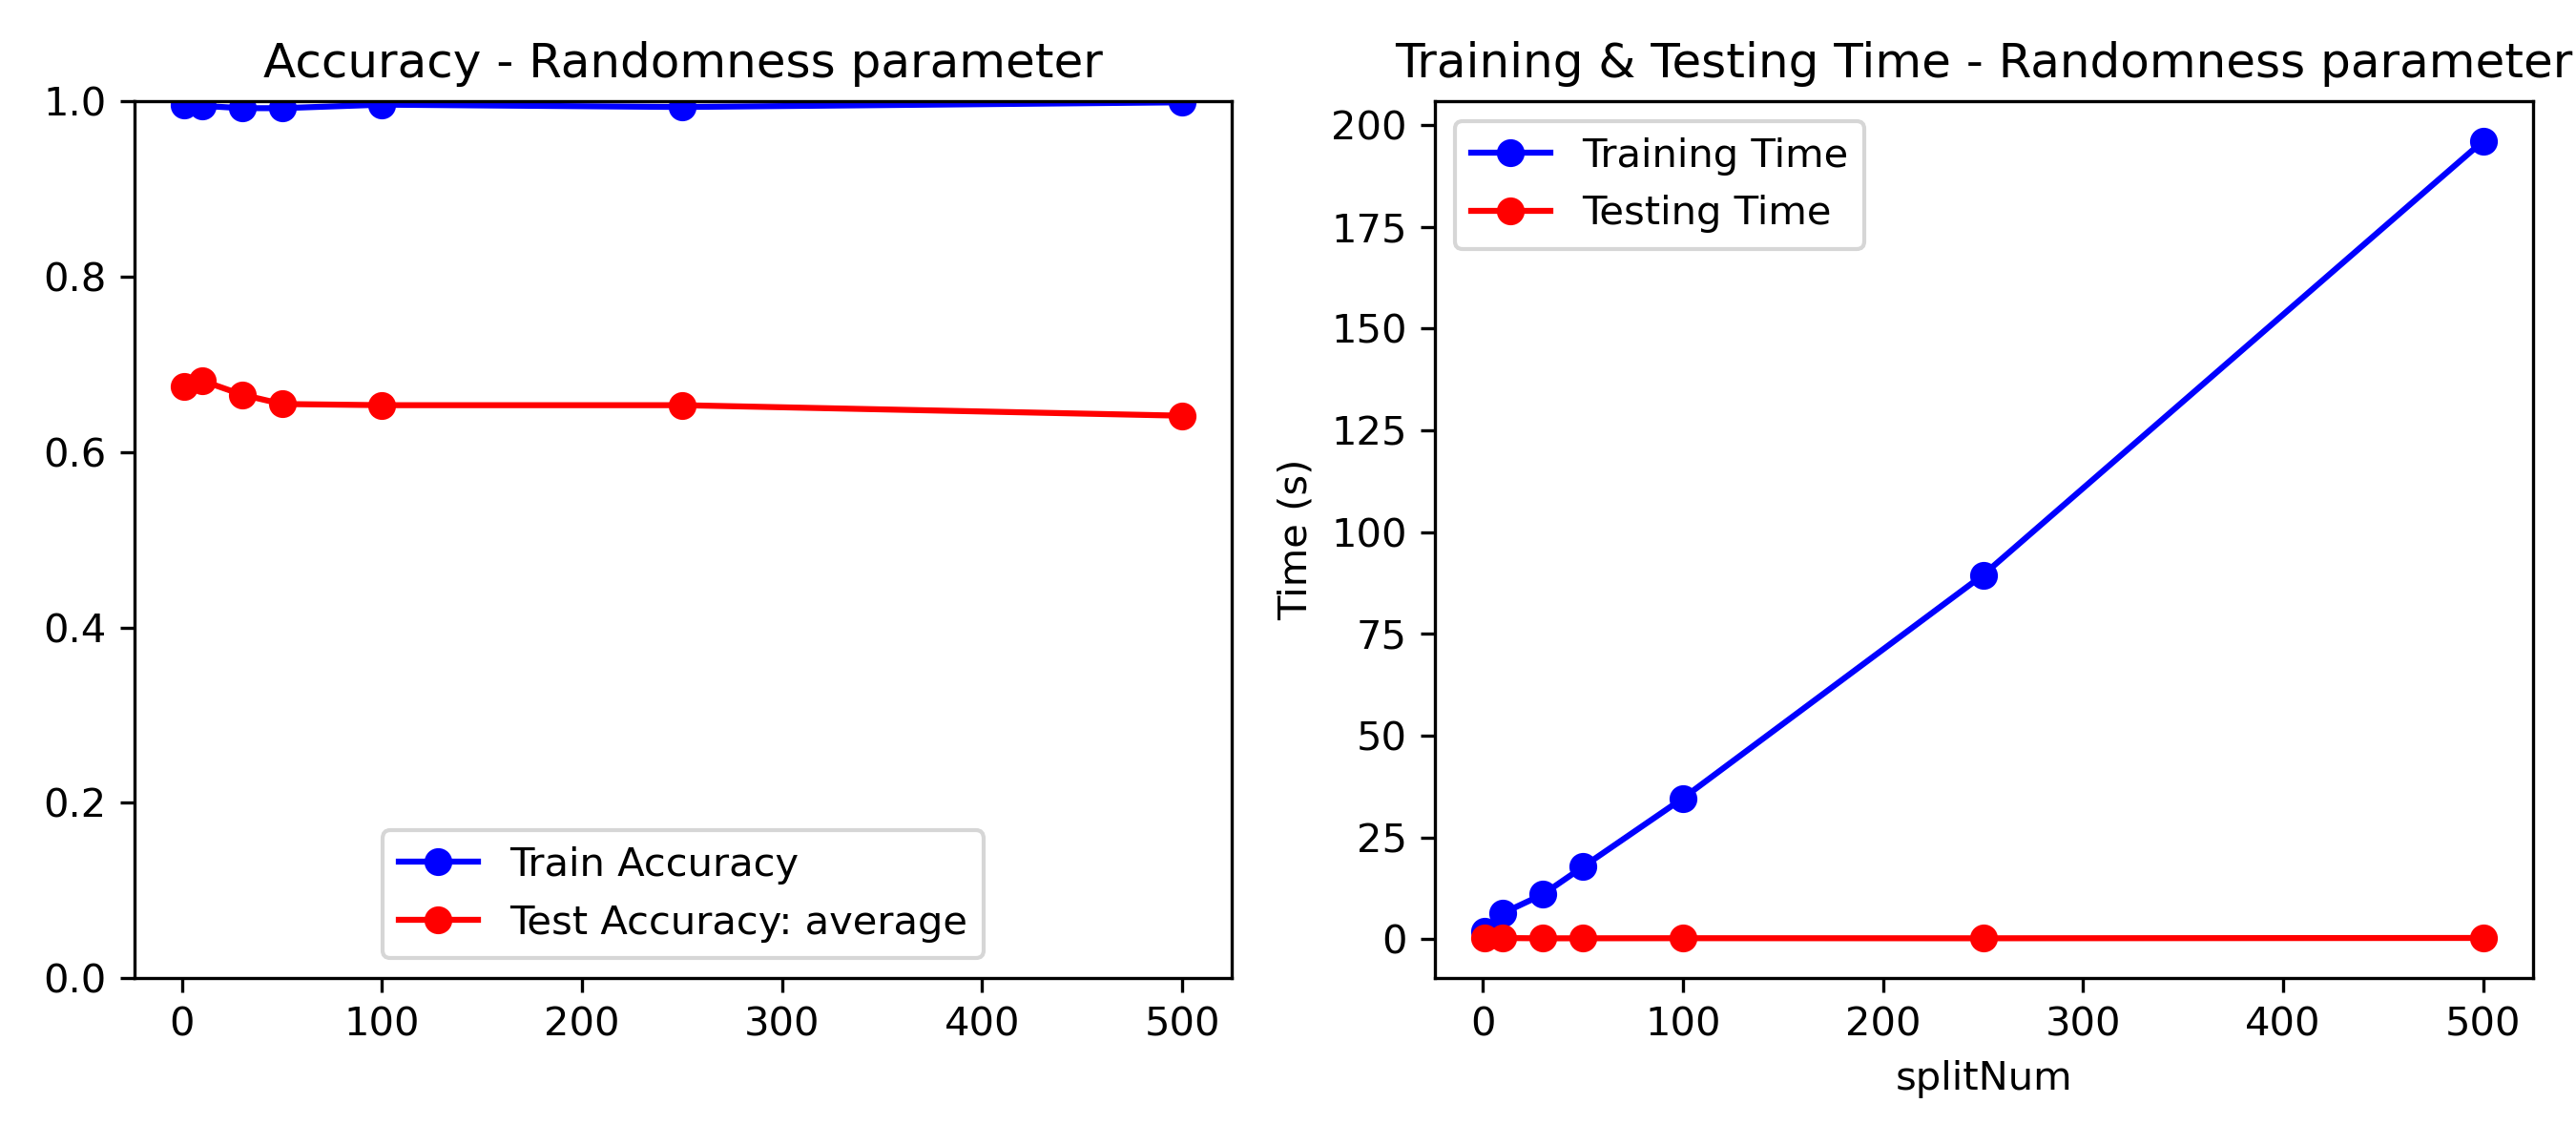
\includegraphics[width=\linewidth]{image/q2-fig4.png}
		\caption{NN-classification face recognition accuracy ($n\_nearest=1$)}
		\label{fig:q2-fig4}
	\end{subfigure}
	\caption{Comparison between Incremental and Batch PCA methods}
	\label{fig:q2}
\end{figure}
\vspace{-0.5cm}
\section{LDA Ensemble for Face Recognition}
\label{sec:intro}

PCA can effectively reduce the dimension of input data preserving important features. And LDA can maximize the variance of between-class while minimize between-class. Thus, using PCA-LDA is expected to increase computing efficiency and classification accuracy. In this section, we try to figure out the effect of PCA-LDA via some experiments.

%-------------------------------------------------------------------------
\subsection{Recognition accuracy of PCA-LDA}

To implement PCA-LDA, we set $M_{pca}$ and $M_{lda}$ by measuring classification accuracy with $M_{pca}$ from 1 to 415 and $M_{lda}$ from 1 to $min(M_{pca}-1, 51)$. This is because, the maximum possible projection dimension for PCA is $N-1$ since the total number of principal components can not be larger than overall data, and for LDA is $n_{class}-1$ since the number of direction for maximizing the distance of between-class and minimizing within-class cannot be larger than the total number of classes. As shown in \cref{fig:mpca_mlda}, accuracy peaked at $M_{pca}=150$ and $M_{lda}=50$. Higher $M_{lda}$ improves performance by enhancing data discrimination, while optimal $M_{pca}$ is between 100 and 200, balancing information retention and overfitting risk.


In LDA, the rank of within-class scatter matrix($S_w$) is $min(364, M_{pca})$, where $N-n_{class}=416-52=364$ and the rank of between-class scatter matrix($S_b$) is $n_{class}-1=51$. Since $\sum_{x\in D_i} (x-m_i) = 0$, each class is linearly dependent, so, $S_w = \sum_{i=1}^c \sum_{x\in D_i} (x-m_i)(x-m_i)^T$ has at most $N-n_{class}$ linearly independent row vectors. After reducing dimensions using PCA, the rank of $S_w$ cannot exceed $M_{pca}$ as the vectors are confined to the PCA subspace. For $S_b$ defined as $S_b = \sum_{i=1}^c (m_i-m)(m_i-m)^T$, it depends only ionly on class means, and since their relationship of class mean does not change after PCA projection since their relationships remain unchanged under PCA (a linear transformation), the maximum possible rank for $S_b$ is $N - n_{class}$.

Based on this observation, we decided to fix $M_{pca}=150$ and $M_{lda}=50$ for further experiments. 

\begin{figure}
  \centering
   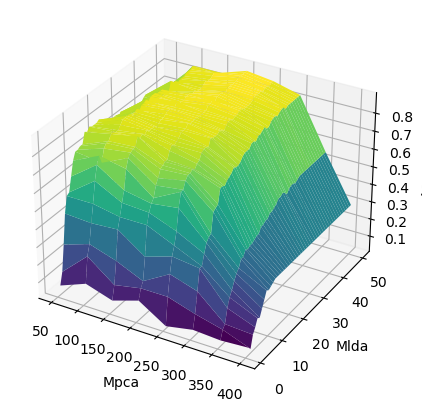
\includegraphics[width=0.8\linewidth]{image/mpca_mlda.png}

   \caption{Classification accuracy varying Mpca and Mlda}
   \label{fig:mpca_mlda}
\end{figure}


%-------------------------------------------------------------------------
\subsection{Result of PCA-LDA}

\cref{fig:q3_1_cm} is the confusion matrix of PCA-LDA classification result. As most of prediction result is on the diagonal entry, it indicates that most of prediction is successful. We take a closer look at success and failure cases. \cref{fig:q3_success} shows successfully predicted cases. Despite the different angles of the faces, the model infer the class accurately. \cref{fig:q3_fail} is failure cases. It seems that the prediction failed because of the similar glasses and face expression.


% %-------------------------------------------------------------------------
% \subsection{Time and Memory}
% Comparison btw pca/pca-lda (accuracy), lda/pca-lda(time), pca/lda/pca-lda(memory)

% %-------------------------------------------------------------------------
% \subsection{PCA-LDA Ensemble}
% For PCA-LDA Ensemble model, we combined two different types of models. The first type is randomization in feature space, which select vectors for pca projection randomly by a certain percentage. The second type is randomization in data sampling, which randomly subsampling the train data by a certain percentage. Both models were used in equal numbers. For combining prediction results of each models, we used 'majority voting' among various fusion rules. This is because, since our task is predicting class for classification and each classes don't have special meaning in numeric value, majority voting looks the most reasonable compared to other methods like averaging and finding maximum. 

%-------------------------------------------------------------------------
\subsection{PCA-LDA Ensemble}
% randomization in feature space (m0)
% randomization in data samples (subset\_rate)
% randomization in model number (model\_num)
% randomness parameter

There are 3 hyperparameter that we can handle randomness: the number of random vector in feature space, the proportion of training data for subsampling, and the number of models for the ensemble. We will examine the impact of each one one by one.

\begin{figure}
	\centering
	\begin{subfigure}[t]{0.48\linewidth}
		\centering
		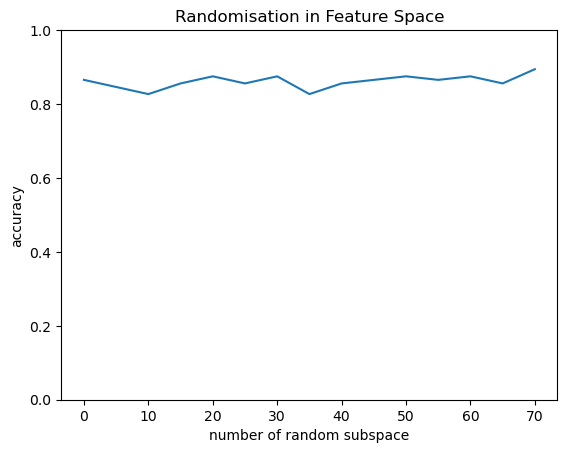
\includegraphics[width=\linewidth]{image/q3_fs_rs.png}
		\caption{Randomization in feature space}
		\label{fig:q3_fs}
	\end{subfigure}%
	\hfill
	\begin{subfigure}[t]{0.48\linewidth}
		\centering
		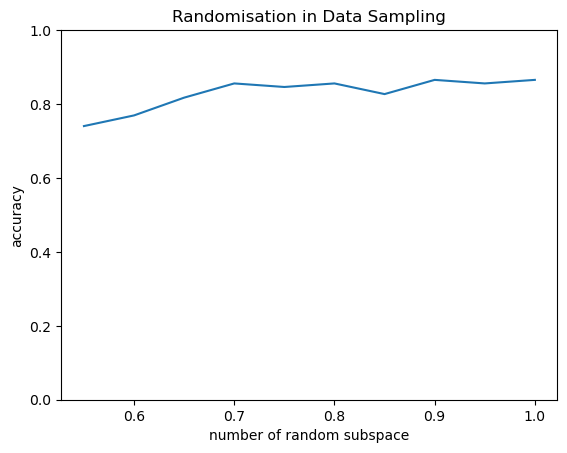
\includegraphics[width=\linewidth]{image/q3_data_rs.png}
		\caption{Random data subsamplint}
		\label{fig:q3_data}
	\end{subfigure}
	
	\begin{subfigure}[t]{0.48\linewidth}
		\centering
		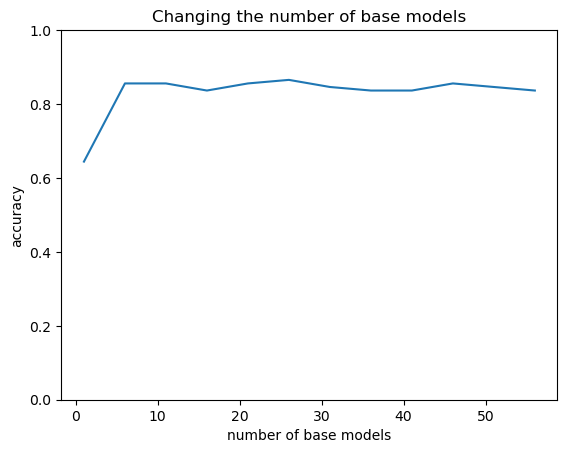
\includegraphics[width=\linewidth]{image/q3_basemodel.png}
		\caption{randomization in the number of basemodels}
		\label{fig:q3_base}
	\end{subfigure}
	\caption{Accuracy comparison between randomness parameters}
	\label{fig:q3_random}
\end{figure}

First, we look into randomization in feature space($M1$). As \cref{fig:q3_fs} indicates, the accuracy is almost highest when the number of random samples is around 30. This is because if the number of random vectors is too large, important features cannot be preserved, and if it is too small, overfitting occurs. Therefore, it is estimated that optimization occurred when the number of random vectors was 30.

Next, we observe the impact of data subsampling proportion($\alpha$). \cref{fig:q3_data} shows the accuracy with respect to the proportion of sub-sampled data. The more data we use, the better accuracy we get. This is quite predictable since the more data you have, the easier it is to generalize.

Lastly, regarding the effect of the number of base models($n_{model}$), we varied the number from 1 to 60, as shown in \cref{fig:q3_base}. When there are fewer than 30 models, the results are similar to a single PCA-LDA model. However, with more than 30 models, performance improves significantly, though further increases beyond 30 yield minimal gains. This is because up to 30 models, the ensemble can capture diverse features for generalization, but the PCA-LDA model’s limited ability to capture complex patterns prevents substantial improvement beyond that point. We used "majority voting" for combining predictions, as it’s most suitable for classification tasks where each class lacks numeric meaning, making it more appropriate than methods like averaging or maximum selection.

Considering both accuracy and computation cost, we conclude that the ensemble model with $M1=30$, $\alpha=0.9$, $n_{model}=30$ has the best performance.

% randomness parameter?

%-------------------------------------------------------------------------
\subsection{Result of PCA-LDA Ensemble}
The accuracy of committee machine, which gather all prediction results from each base models from ensemble model, is 0.846. And the average of individual models in ensemble model is 0.736. From this result, we can check that the performance of committee machine is better than individual as we learned. (Ensemble Learning LN, p.11-13)

In addition, \cref{fig:q3_2_cm} shows the confusion matrix of ensemble model. Compared to \cref{fig:q3_1_cm}, since \cref{fig:q3_2_cm} has less components outside the diagonal, we can visually check that the accuracy of classification of ensemble model is higher than single PCA-LDA model.

\section{Convolutional Neural Networks}
\label{sec:intro}

%-------------------------------------------------------------------------
\subsection{CNN architecture}
Our default CNN architecture is as below: 
\begin{itemize}
	\item 4 convolutional layers with ReLU and Maxpooling
	\item 4 fully connected layers with drop-out and ReLU
	\item Residual connections to every one layers
	\item Use CrossEntropy as a loss function for optimization
	\item The size of convolutional filter size 3
\end{itemize}
In addition, the input of our CNN is resized to 128*128 since Caltech101 dataset has image sizes 100 to 300. Detailed architecture including the dimension of channels are in \cref{fig:cnn_arch}. We tried to choose simple and high-performance model.
\begin{figure}[htbp]
	\centering
	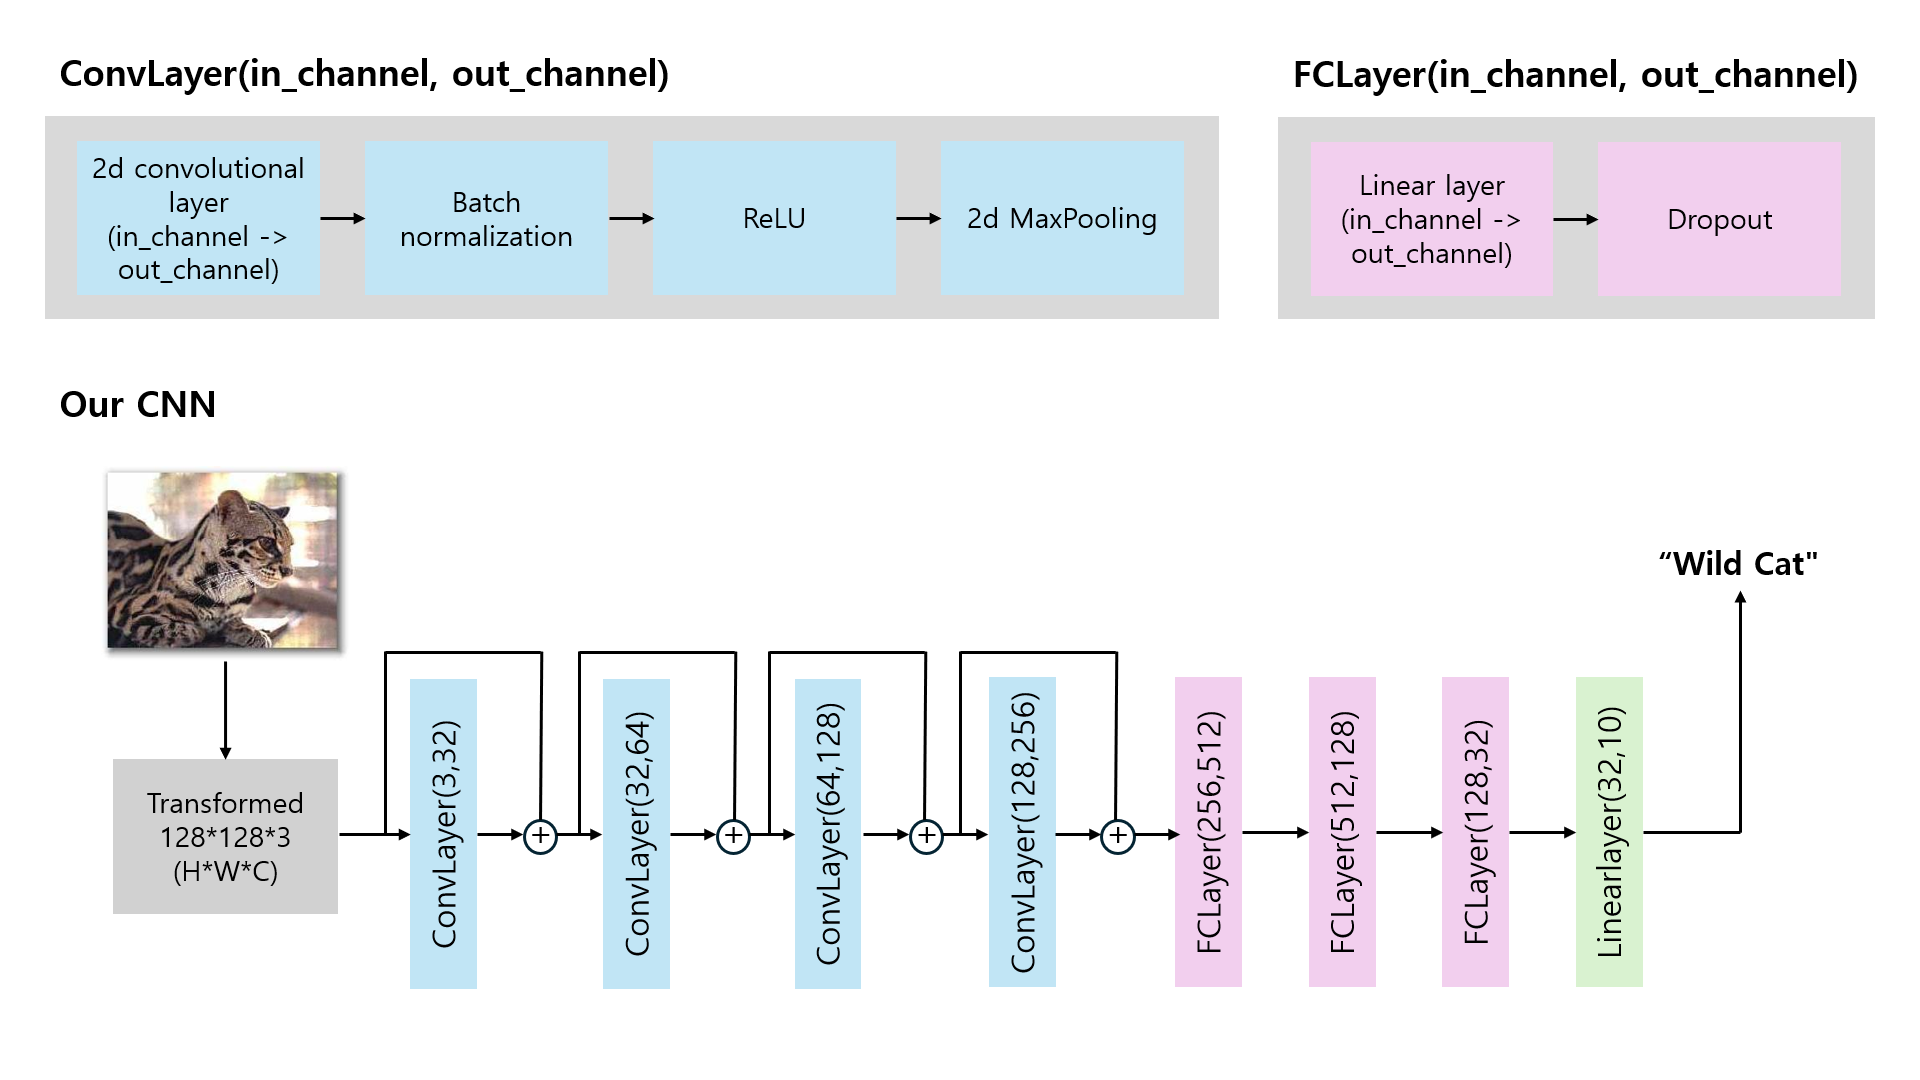
\includegraphics[width=0.7\linewidth]{image/q4-1-arch.png}
	\caption{Our CNN architecture}
	\label{fig:cnn_arch}
\end{figure}

\subsection{Changing architecture}
We changed the number of layers from 3 to 5. As shown in \cref{fig:q4-2-layers}, the test accuracy is highest with 4 layers. When CNN has 3 layers, it is not enough to extract useful features from images. Also when it has 5, we expected over-fitting due to the gradient vanishing. Hence, we selected 4 layers would be the best choice for performance.

Next, we changed the size of kernel to 3, 5, and 7. As \cref{fig:q4-2-kernel} shows, the accuracy is highest when the kernel size is 3 and it decreases afterwards. When the kernel size is small, it is adequate to capture the details of images and when the size is big, it is good to perceive the global scene. However, as our image has 128*128 size, which is small, kernel size 3 is enough to extract useful feature of the image since we also used residual connections. Other sizes might be too big to recognize the detailed features.

Finally, we investigate the effect of residual connections between layers. There are three cases: no connections, connections between every two layers, and connections between each layer. With 4 layers in total, the number of connections are 0, 2, and 4, respectively. The test accuracy, shown in \cref{fig:q4-2-connection}, increases with the number of connections. This improvement is due to the residual connections, which prevent information loss from the initial layers, allowing the CNN to learn more various hierarchical features of the images and their labels.

\begin{figure}[htbp]
	\centering
	\begin{subfigure}[t]{0.3\linewidth}
		\centering
		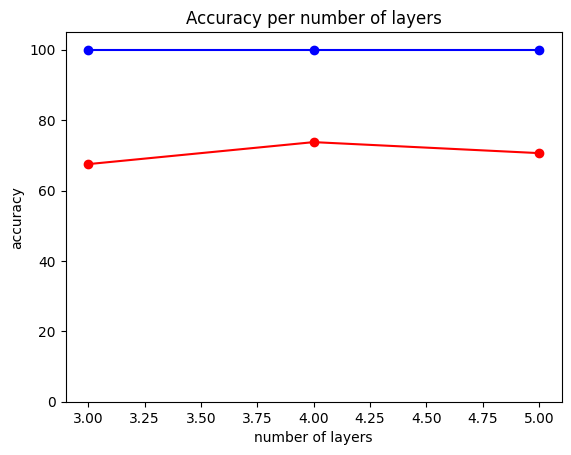
\includegraphics[width=\linewidth]{image/q4-2-layers.png}
		\caption{Accuracy according to layers}
		\label{fig:q4-2-layers}
	\end{subfigure}	
    \hfill
	\begin{subfigure}[t]{0.3\linewidth}
		\centering
		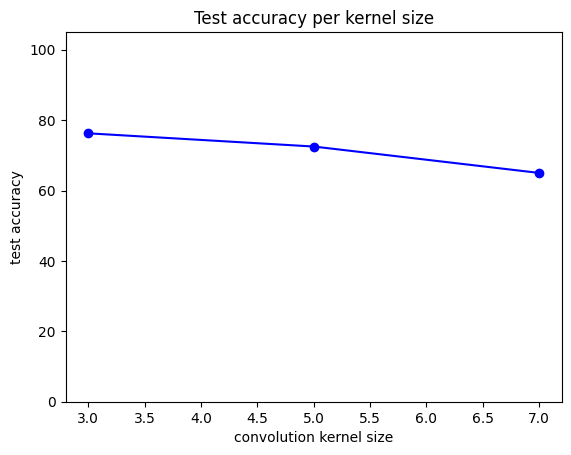
\includegraphics[width=\linewidth]{image/q4-2-kernel.png}
		\caption{Accuracy according to kernel size}
		\label{fig:q4-2-kernel}
	\end{subfigure}%
    \hfill
	\begin{subfigure}[t]{0.3\linewidth}
		\centering
		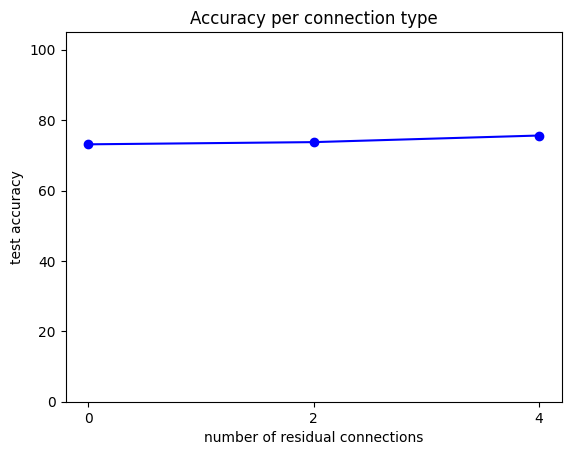
\includegraphics[width=\linewidth]{image/q4-2-connection.png}
		\caption{Accuracy according to connections}
		\label{fig:q4-2-connection}
	\end{subfigure}

	\caption{impact of changing architecture of CNNs}
	\label{fig:cnn_architecture}
\end{figure}

\subsection{Layer normalization}
To explore the effect of the layer normalization method, we tested our model using 4 different methods: batch, layer, instance, and group normalization.

The accuracies according to the batch number for each method are shown in \cref{fig:normalization}. We can check that batch normalization is greatly affected by the size of batch, while the others show consistent accuracy w.r.t. the size of the batch. For batch normalization, batch size increases improve accuracy up to a size of 16. This is because larger batches result in a smoother convergence and stable gradient values. However, too large batch can reduce accuracy due to the diminishing of generalization, as small batch sometimes introduces randomness.

In image classification, it is important to catch the difference between feature distribution of within and between classes. Using batch normalization, we can consider class distribution since the normalization is performed on a batch basis. However, other methods only do normalization within a single image, the information related to class statistics is weakened. Hence, their accuracy becomes lower than using batch normalization. Also, in layer normalization paper\cite{ba2016layernormalization}, they mentions that it is worse than batch normalization in simple CNN model.

\begin{figure}
	\centering
	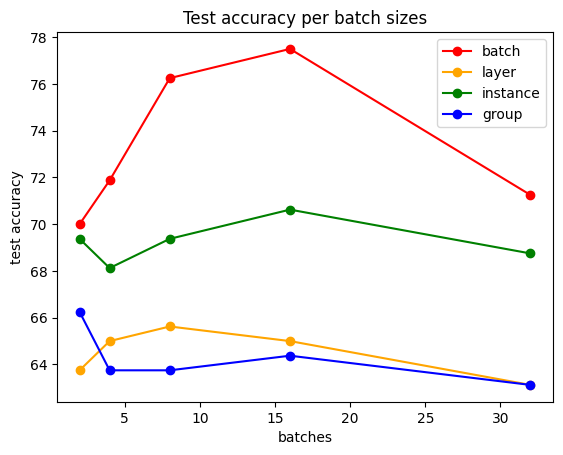
\includegraphics[width=0.4\linewidth]{image/q4-3.png}
	\caption{Accuracy according to normalization types}
	\label{fig:normalization}
\end{figure}

\subsection{Generalization}
In this section, we are going to check the impact of drop-out and L2-regularization term(which is in Deep\_Learning\_intro Lecture Note pg.84). We tested our basic model which has drop-out, the model without drop-out, and the model with L2-regularization on weights. Results are shown in \cref{table:generalization}. The model without generalization method has the lowest accuracy and the model with L2-regularization has the highest accuracy. This is because, dropout randomly deactivate some neurons, so it helps model to avoid overfitting and be good at generalization. And L2-regularization helps model to avoid overfitting by regulate the size of weights.

\begin{table}
	\centering
	\setlength{\tabcolsep}{6pt}
	\renewcommand{\arraystretch}{1.5}
	\resizebox{0.5\linewidth}{!}{
		\begin{tabular}{|c||c|}
		\hline
		& accuracy  \\ \hline\hline
		original & 75.625  \\ \hline
		without dropout & 68.125  \\ \hline
		with L2-regularization term & 76.250  \\ \hline
		\end{tabular}
	}
    \caption{Impact of generalization}
	\label{table:generalization}
\end{table}
	

\subsection{Loss function}
We used CrossEntropy, based on the softmax function, as the default loss function. In this section, we compare it with the SquaredHinge loss. Using CrossEntropy, we achieved 73.75\% accuracy, while SquaredHinge gave a higher accuracy of 80.00\%. This improvement is due to the fact that CrossEntropy relies on probability distribution, while SquaredHinge focuses on the margin between predicted and true classes. Given the small size of our dataset (10 classes), estimating an accurate probability distribution is challenging due to the law of large numbers. Thus, SquaredHinge, which directly considers class margins, performs better. Nevertheless, we utilized CrossEntropy as the default option due to its widespread use.


\subsection{Compressing CNN}
We conduct an experiment on compressing CNN layers using truncated SVD. Our model has 4 fully connected layers with ranks 512, 128, 32, and 10, and we compress the first two layers by 100\% (original), 75\%, 50\%, and 25\% because the last two layers are too small to compress. The result is shown in \cref{fig:cnn_svd}. As expected, a tradeoff between accuracy and efficiency is observed, since compressing the weight matrices improve both time and space-wise efficiency but generate information loss.

\begin{figure}
	\centering
	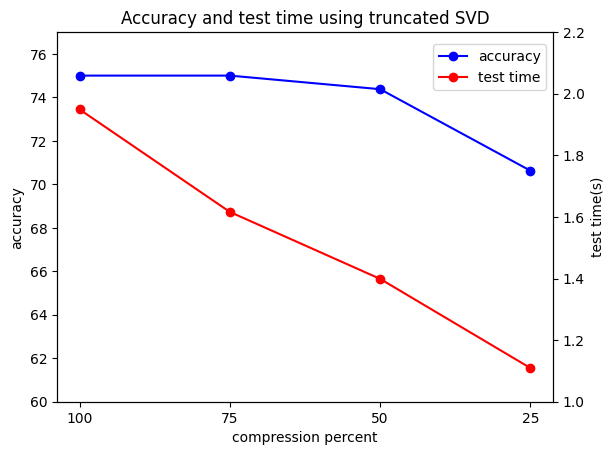
\includegraphics[width=0.4\linewidth]{image/q4-6-svd.png}
	\caption{Accuracy and test time using truncated SVD}
	\label{fig:cnn_svd}
\end{figure}

\subsection{Changing parameters}
We observe the effect of 3 main hyperparameters: learning rate, batch size, and the number of epochs.

\cref{fig:q4-7-lr-train} and \cref{fig:q4-7-lr} show the results of varying the learning rate. We experimented with learning rates of 0.00001, 0.0001, 0.0005, and 0.005. When the learning rate is 0.00001, the model does not reach the local minima, as it is converges very slow. For learning rates of 0.0005 and 0.001, the model oscillates excessively before converging, with the amplitude of oscillation being larger at 0.001 than at 0.0005. This happens because the step size is too large, causing the model to overshoot the local minimum. Therefore, we determined that a learning rate of 0.0001 is optimal for our model. Also, the highest accuracy is achieved at a learning rate of 0.0001, while smaller or larger learning rates result in lower accuracy. 

We trained our model with batch sizes ranging from $2^1$ to $2^6$ and achieved the highest accuracy with a batch size of 16 as in \cref{fig:q4-7-batch}. With small batch sizes, the model learns feature distributions from a limited amount of data, leading to noisy gradient and less smooth converging. However, such noise can allow the model to explore the loss landscape more broadly, helping generalization. This might help the optimizer avoid getting stuck in local minima or saddle points. Therefore, our optimal batch size was 16 because of such tradeoff. In general, we can conclude that using mini-batch rather than whole-data gradient can reduce the training time and offers better monitoring progress.

For the number of epochs, results are shown in \cref{fig:q4-7-epoch}. The accuracy is the highest with 100 epochs because when the number of epoch is not enough, it can cause under-fitting and if there is too much epoch, it can cause over-fitting.

\begin{figure}
	\centering
	\begin{subfigure}{0.23\linewidth}
		\centering
		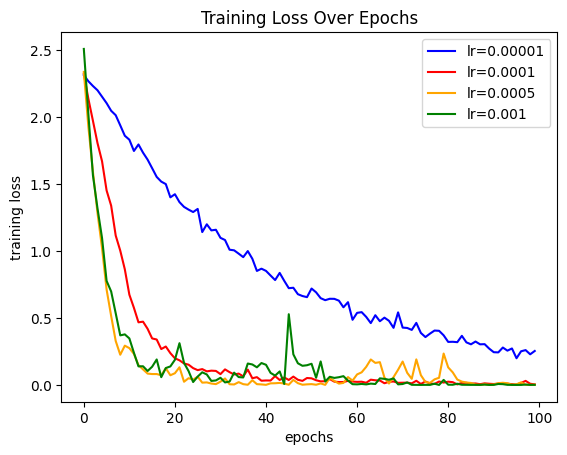
\includegraphics[width=\linewidth]{image/q4-7-lr-train.png}
		\caption{Learning rate training losses}
		\label{fig:q4-7-lr-train}
	\end{subfigure}%
	\hfill
	\begin{subfigure}{0.23\linewidth}
		\centering
		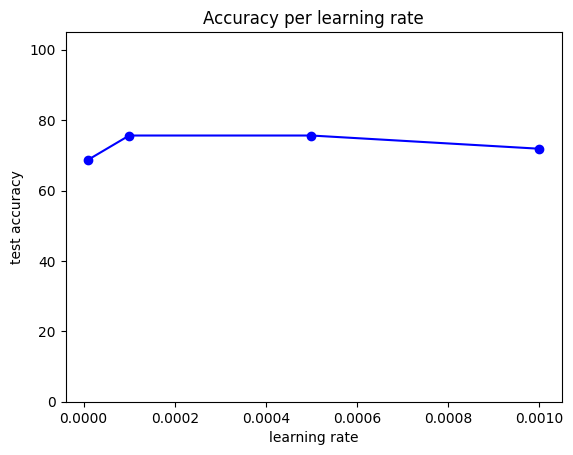
\includegraphics[width=\linewidth]{image/q4-7-lr.png}
		\caption{Learning rate accuracy}
		\label{fig:q4-7-lr}
	\end{subfigure}
	\hfill
	\begin{subfigure}{0.23\linewidth}
		\centering
		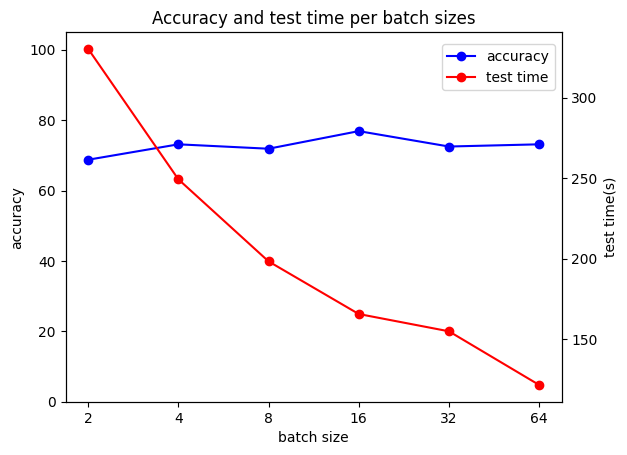
\includegraphics[width=\linewidth]{image/q4-7-batch.png}
		\caption{Batch size accuracy}
		\label{fig:q4-7-batch}
	\end{subfigure}
	\hfill
	\begin{subfigure}{0.23\linewidth}
		\centering
		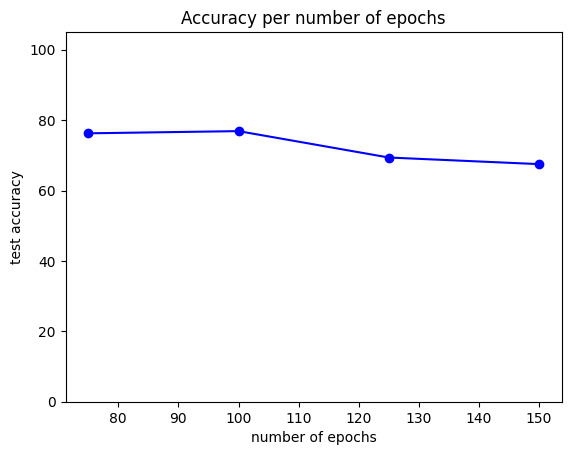
\includegraphics[width=\linewidth]{image/q4-7-epoch.png}
		\caption{Epoch accuracy}
		\label{fig:q4-7-epoch}
	\end{subfigure}
	\caption{Changing hyper-parameters of CNN}
	\label{fig:q2}
\end{figure}

\subsection{Pre-trained model}
We compared two initialization methods: fine-tuning pre-trained weight model and training from random initialization. For this experiment, we used pre-trained ResNetModel(microsoft/resnet-50, trained with ImageNet)\cite{ref1} and fine-tuned it with Caltech101 dataset. Due to our limited computing resource, we only train it with 10 epochs. When we use pre-trained weights and fine-tuned them, we get 99.33\% accuracy while training from scratch represents 21.33\%. Based on this result, the initialization weight highly affects the deep learning's convergence. It is because, since our pre-trained weights are obtained from performing same task(image classification) with large dataset, such initialization weights already have some useful features for image classification. 

\subsection{Comparison with other methods}
Our CNN model's accuracy is about 75\%, which is better than Q2 and Q3 as shown in \cref{table:accuracy}. This is because CNN can do end-to-end learning from feature extraction to classification, unlike Q2 and Q3's model. In other words, k-means or random forest vocabulary followed by random forest classification does not allow end-to-end learning, making it difficult to determine whether the vector quantisation result includes beneficial features for classification. However, CNN can automatically learn various meaningful representations directly from raw data.

\begin{table}[htbp]
	\centering
	\setlength{\tabcolsep}{6pt} % Adjust column spacing
	\renewcommand{\arraystretch}{1.5} % Adjust row height
	\resizebox{0.5\textwidth}{!}{ % Scale table to fit text width
		\begin{tabular}{|c||c|c|}
			\hline
			& Train Accuracy (\%) & Test Accuracy (\%) \\ \hline\hline\
			K-means Codebook - RF Classifier & 99.50 & 68.5   \\ \hline
			RF Codebook - RF Classifier & 97.80 & 60.67  \\ \hline
			CNN & 100.00 & 75.625  \\ \hline
		\end{tabular}
	}
	\caption{Accuracy of Models}
	\label{table:accuracy}
\end{table}
\section{RF classifier}
\label{sec:intro}

The random forest model has several key parameters, and testing them all simultaneously would require excessive effort and time. Therefore, we configured the optimal parameters in the sequence described below. Also, to ensure result stability, each test was executed 10 times, with the average result displayed in a graph, and the confusion matrix representing the best result among the 10 runs is recorded in Appendix.
\begin{enumerate}
	\item Number of Trees \& Tree Depth: We tested using an axis-aligned weak learner with the split number fixed at 10.
	\item Split Number (Randomness Parameter): Using the optimal number of trees and tree depth derived in step 1, with an axis-aligned weak learner.
	\item Type of Weak Learner: With the optimal values for other parameters determined in steps 1 and 2, we tested different weak learners.
\end{enumerate}

%-------------------------------------------------------------------------
\subsection{Number of trees \& The depth of trees}
We varied the number of trees and their depths, obtaining the results shown in \cref{fig:q5-fig1}. In the graph, the best accuracy 0.625 occurred at $N(number of trees)=250$ and $D(depth)=10$, explained as follows:
\begin{itemize}
	\item Number of Trees: A single tree in random forests tends to overfit to data; therefore, we can generalize the model using ensembles of trees. As shown in \cref{fig:q5-fig1}, the accuracy converges near $N=250$, which is selected as optimal parameter.
	\item Tree Depth: When depth is $D$, maximum of $2^D-1$ nodes are generated. As shown in \cref{fig:q5-fig1}, for a given $N$, accuracy initially increases with tree depth but later decreases due to overfitting. Notably, the optimal depth $D$ increases with $N$, indicating that a larger $N$ result in less overfitting. Also, we chose $D=8$ as the later experiment's standard value, accuracy of 0.610, which is sufficiently high.
\end{itemize}

The theoretical training/testing time when adjusting the number of trees and tree depth is as follows, and our testing time results align with theoretical predictions \cref{fig:q5-fig2}, \cref{fig:q5-fig3}. However, due to the small size of the training data, some splits stop prematurely, not reaching the maximum tree depth, resulting in  less training time than theory.
\begin{itemize}
	\item Number of Trees $N$: $O(N)$ time
	\item Tree Depth $D$: $O(2^D)$ time
\end{itemize}
Moreover, our code do not utilize parallelization of each tree's growth. Based on theoretical insights from course materials, training each tree in parallel could reduce the time for the tree numbers to $O(1)$, not $O(N)$.

\begin{figure}
	\centering
	\begin{subfigure}[t]{\linewidth}
		\centering
		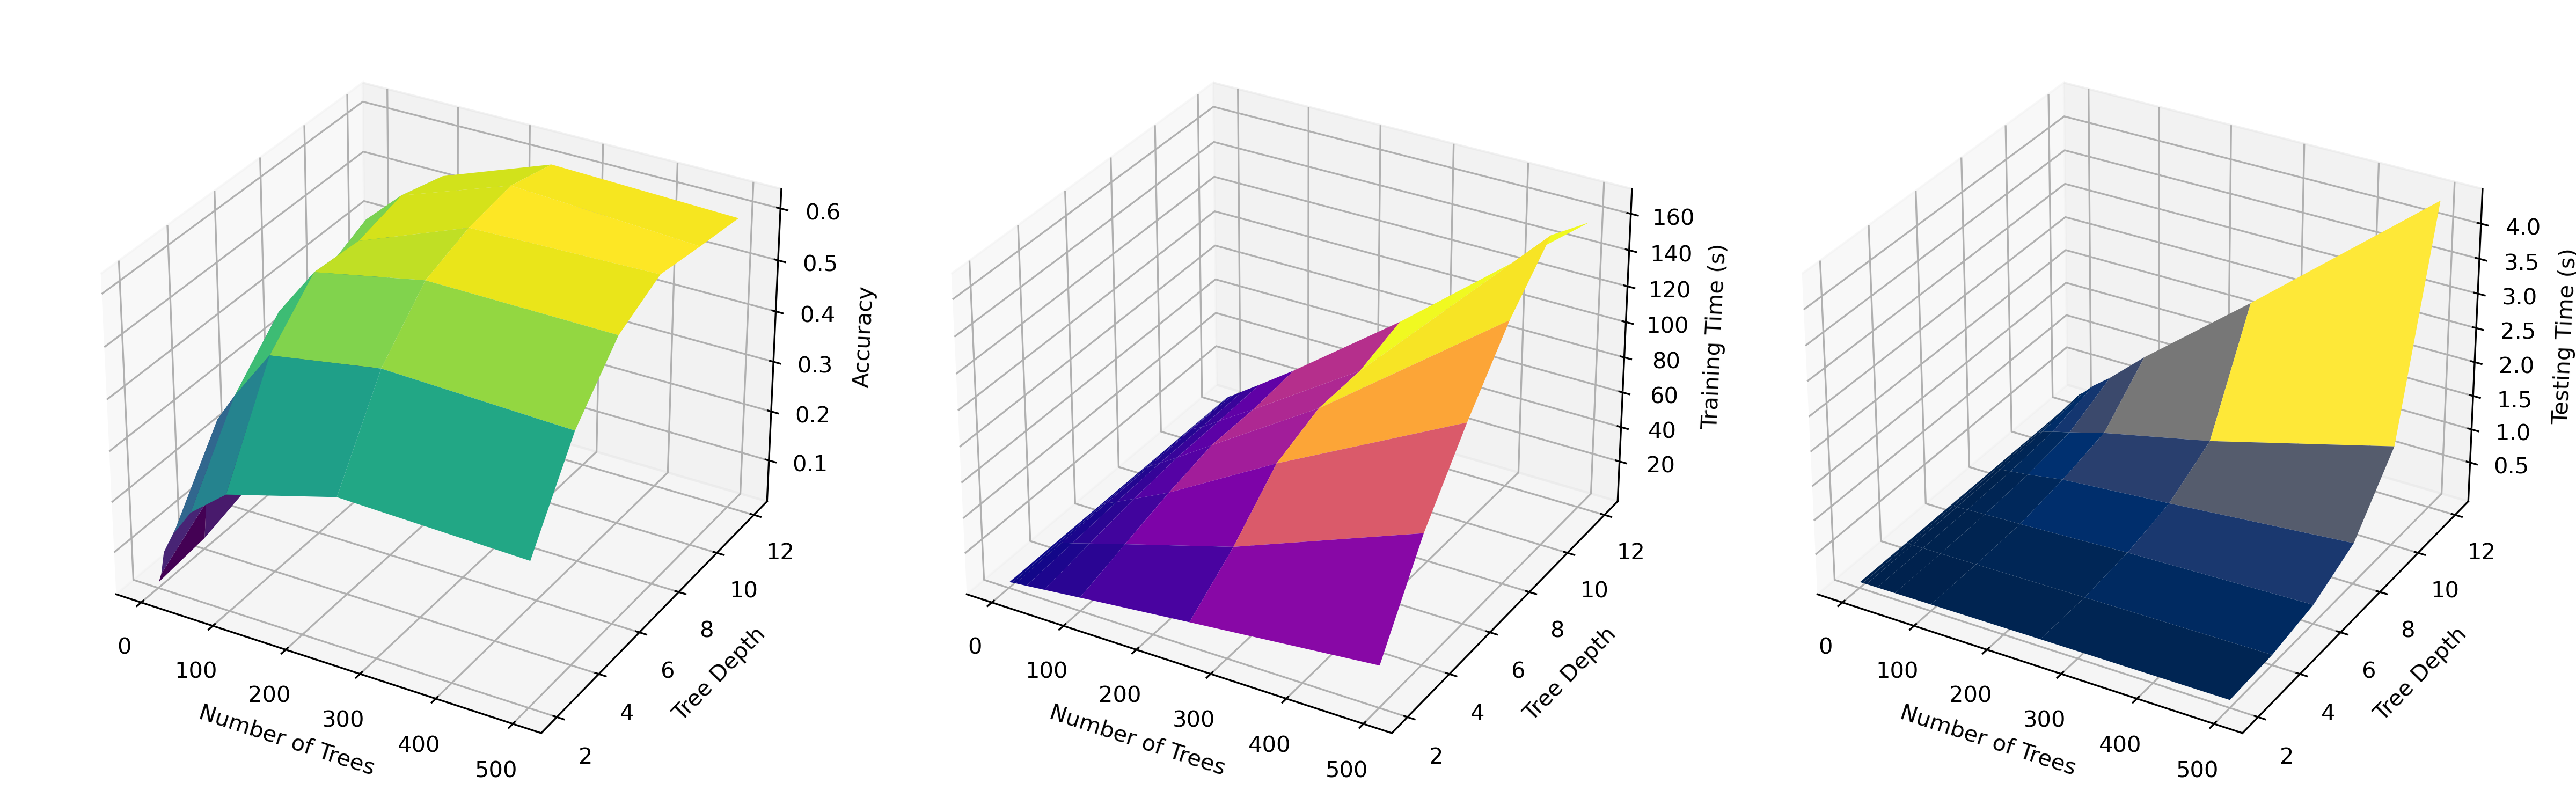
\includegraphics[width=\linewidth]{image/q5-fig1.png}
		\caption{Test accuracy, Training time, Testing time according to the number of tree and the depth of tree}
		\label{fig:q5-fig1}
	\end{subfigure}
	\begin{subfigure}[t]{\linewidth}
		\centering
		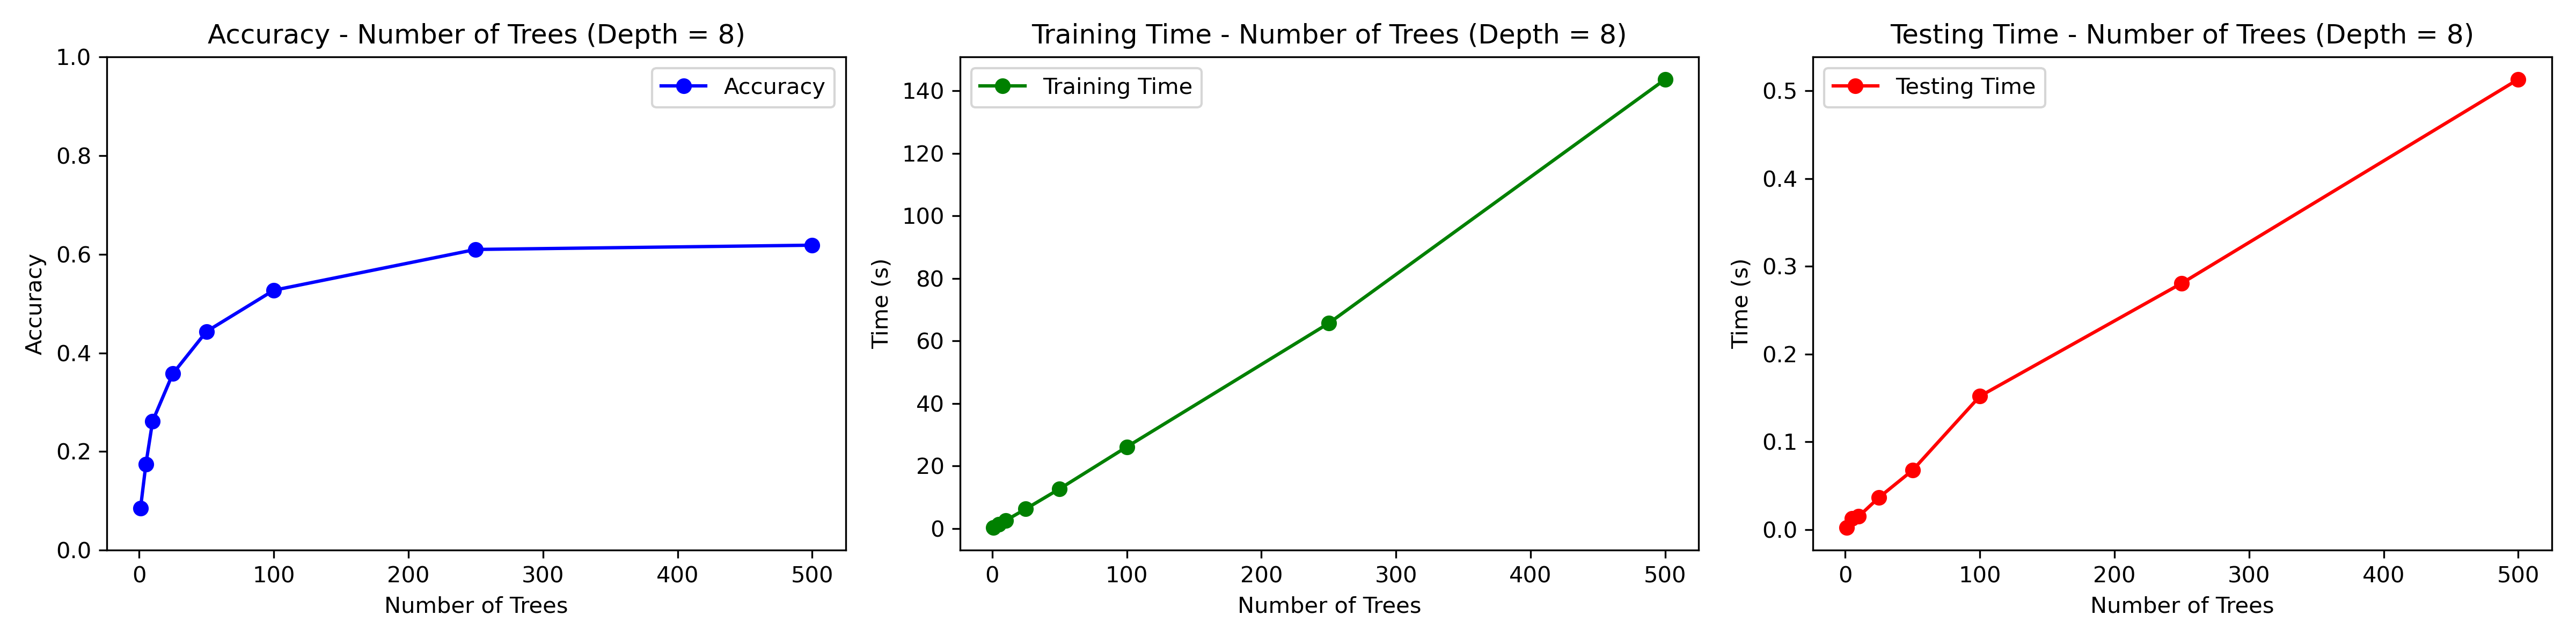
\includegraphics[width=\linewidth]{image/q5-fig2.png}
		\caption{Test accuracy, Training time, Testing time according to the number of tree (D = 8)}
		\label{fig:q5-fig2}
	\end{subfigure}
	\begin{subfigure}[t]{\linewidth}
		\centering
		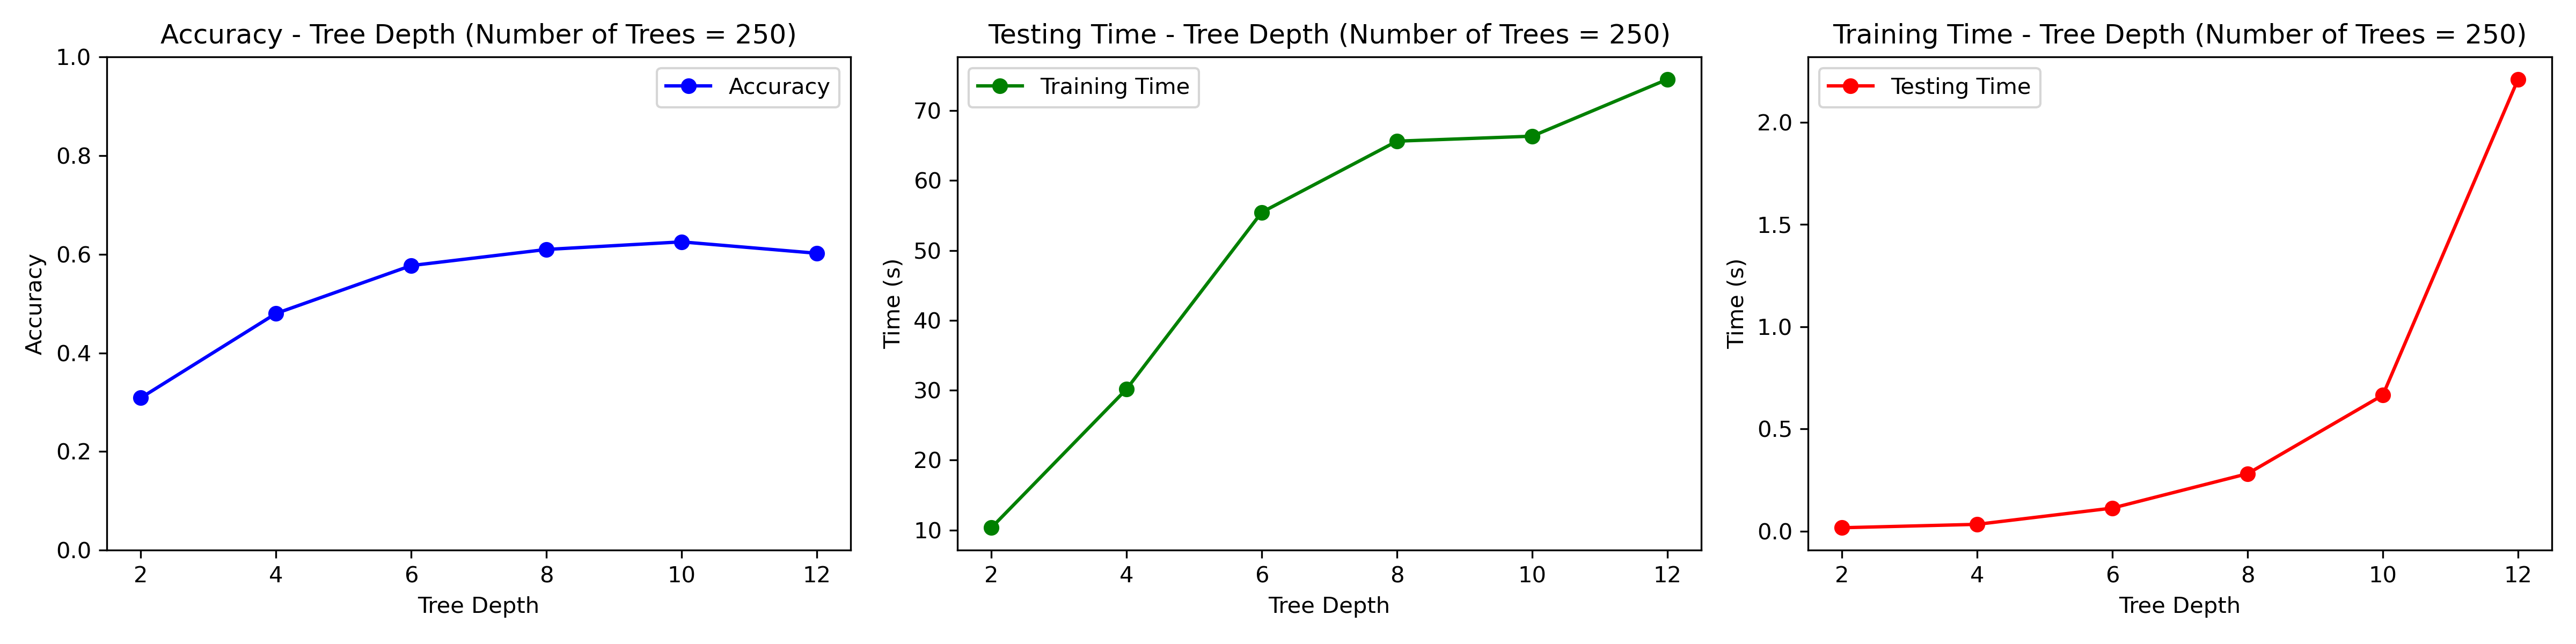
\includegraphics[width=\linewidth]{image/q5-fig3.png}
		\caption{Test accuracy, Training time, Testing time according to the depth of tree (N = 250)}
		\label{fig:q5-fig3}
	\end{subfigure}
	\caption{Test accuracy, training/testing time according to the number and depth of trees}
\end{figure}

\subsection{Randomness parameter}
Due to the high dimension image data, we randomly select dimensions and threshold values to create the split function. For each split function, we attempt $\rho$ random splits and choose the one with the highest information gain. There is a trade-off in the magnitude of $\rho$ value: If the $\rho$ value is too low, fewer splits are attempted, which reduces similarity between trees but increases the risk of the less-optimal split. Conversely, as $\rho$ increases, more various split functions are tested, leading to greater similarity among trees, which decreases the advantage of ensemble multiple trees. As shown in \cref{fig:q5-fig4}, accuracy initially increases with higher $\rho$ values until $\rho=10$ and then decreases, as expected. In \cref{fig:q5-fig5}, training time is same as expected, $O(\rho)$. However, since $\rho$ does not affect the resulting tree structure in training, it has constant testing time.

\begin{figure}
	\centering
	\begin{subfigure}[t]{0.4\linewidth}
		\centering
		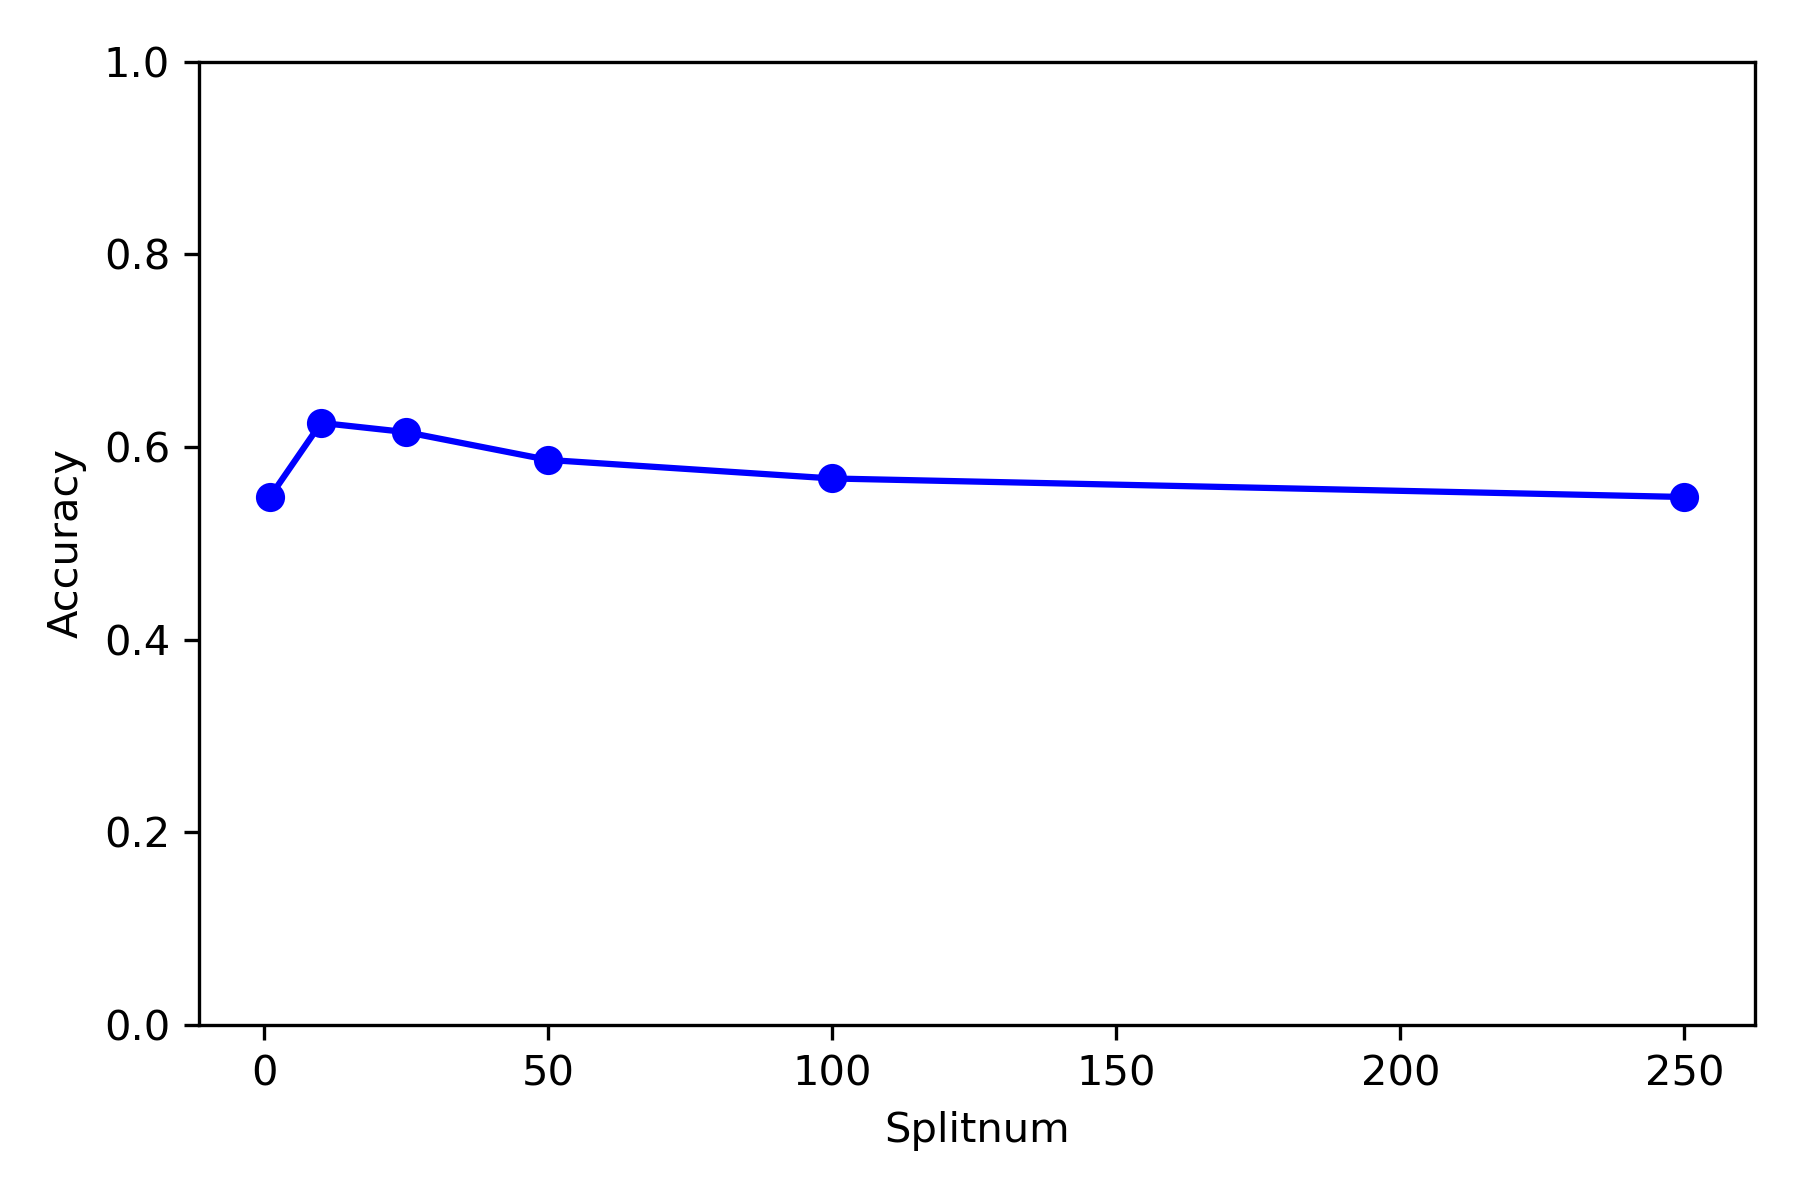
\includegraphics[width=\linewidth]{image/q5-fig4.png}
		\caption{Test accuracy according to the randomness parameter}
		\label{fig:q5-fig4}
	\end{subfigure}%
	\quad
	\begin{subfigure}[t]{0.4\linewidth}
		\centering
		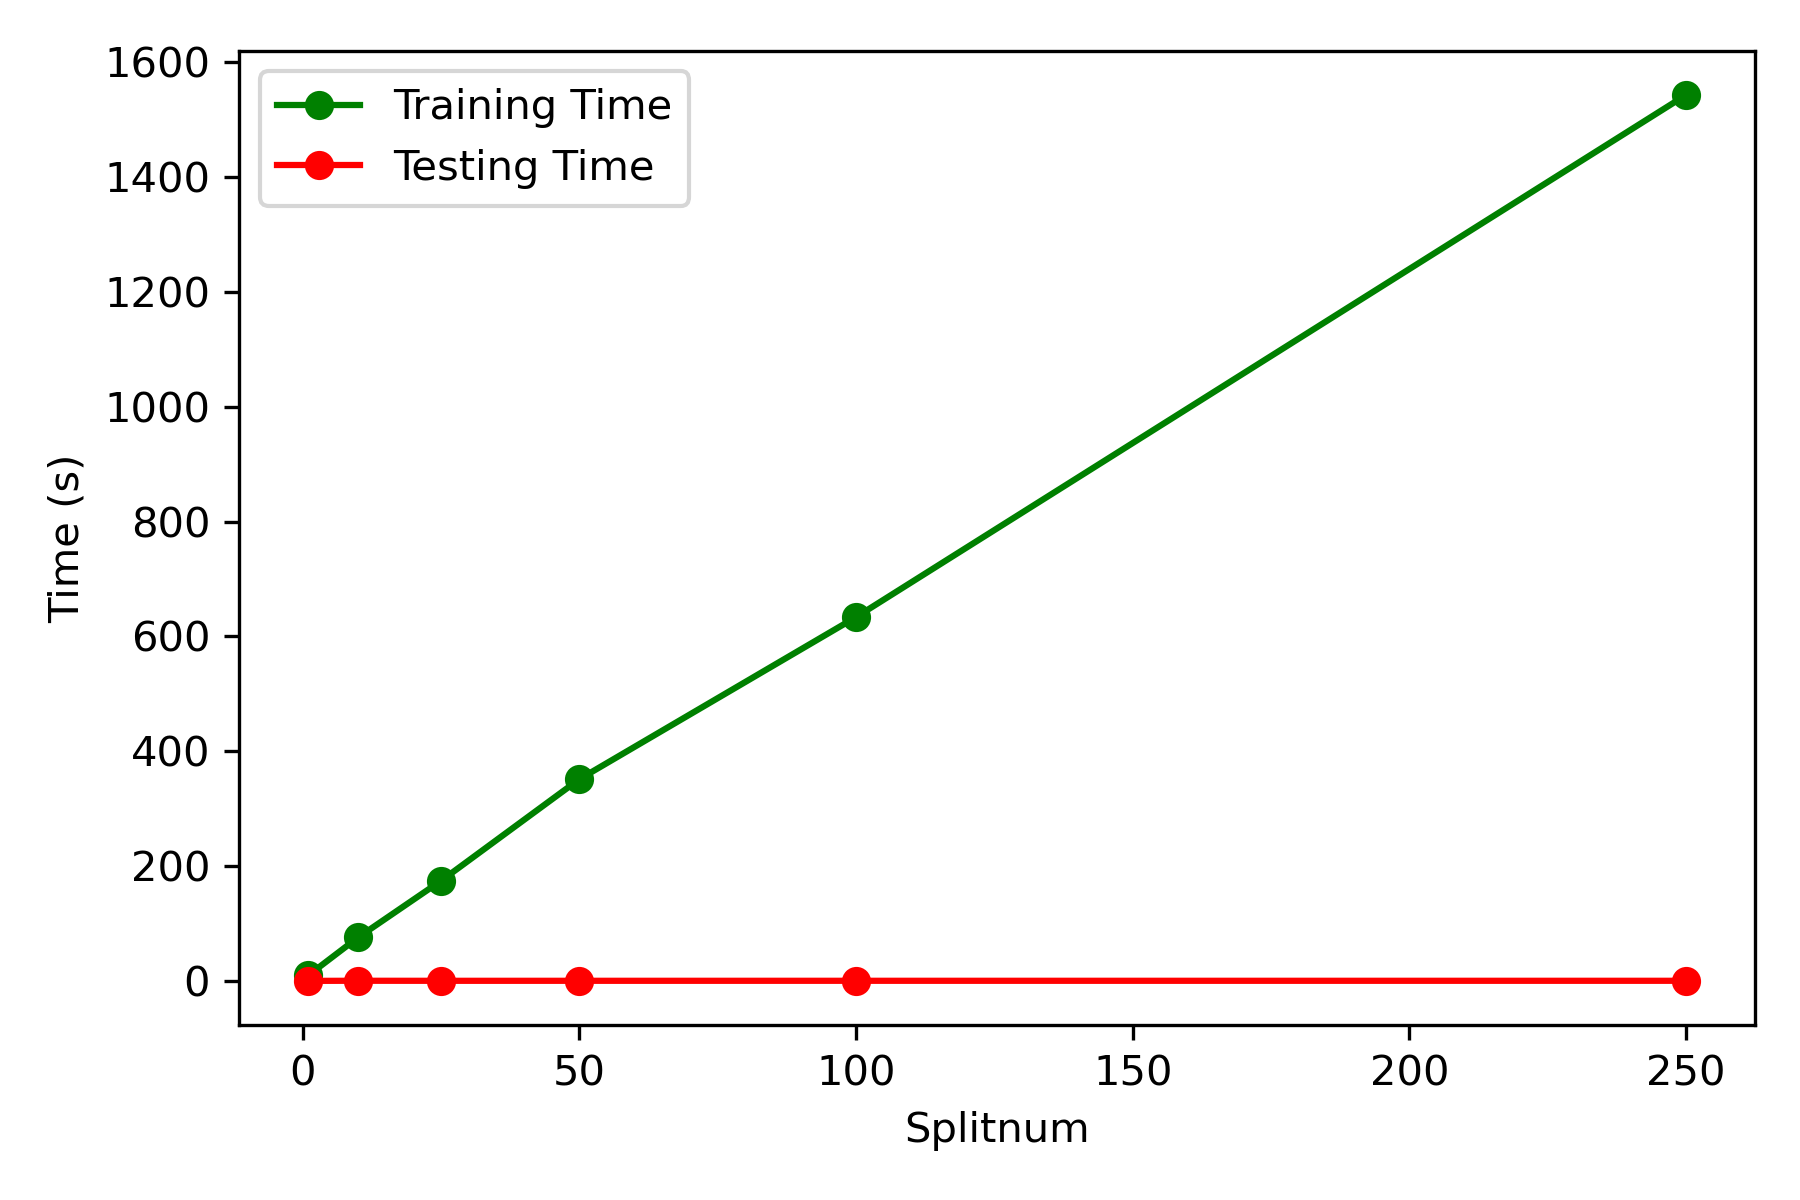
\includegraphics[width=\linewidth]{image/q5-fig5.png}
		\caption{Training time, Testing time according to the randomness parameter}
		\label{fig:q5-fig5}
	\end{subfigure}
	\caption{Test accuracy, training/testing time according to the randomness parameter}
\end{figure}

\subsection{Impact of the different types of weak-learners}
The impact of the weak learner are shown in \cref{fig:q5-fig7}. As expected, the axis-aligned method provides sufficiently good testing accuracy along with the shorter training and testing times. However, even with all other parameters being the same, the accuracy when using the two-pixel test is approximately 8.32\% higher. Therefore, the two-points test's information gain per split is greater than that of the axis-aligned method. Although other weak learners, such as linear and non-linear methods, were also implemented and tested, they took so long to measure training and testing times that it was expected impractical for real-time training/testing, and thus they were not included in the report.
\begin{figure}
	\centering
	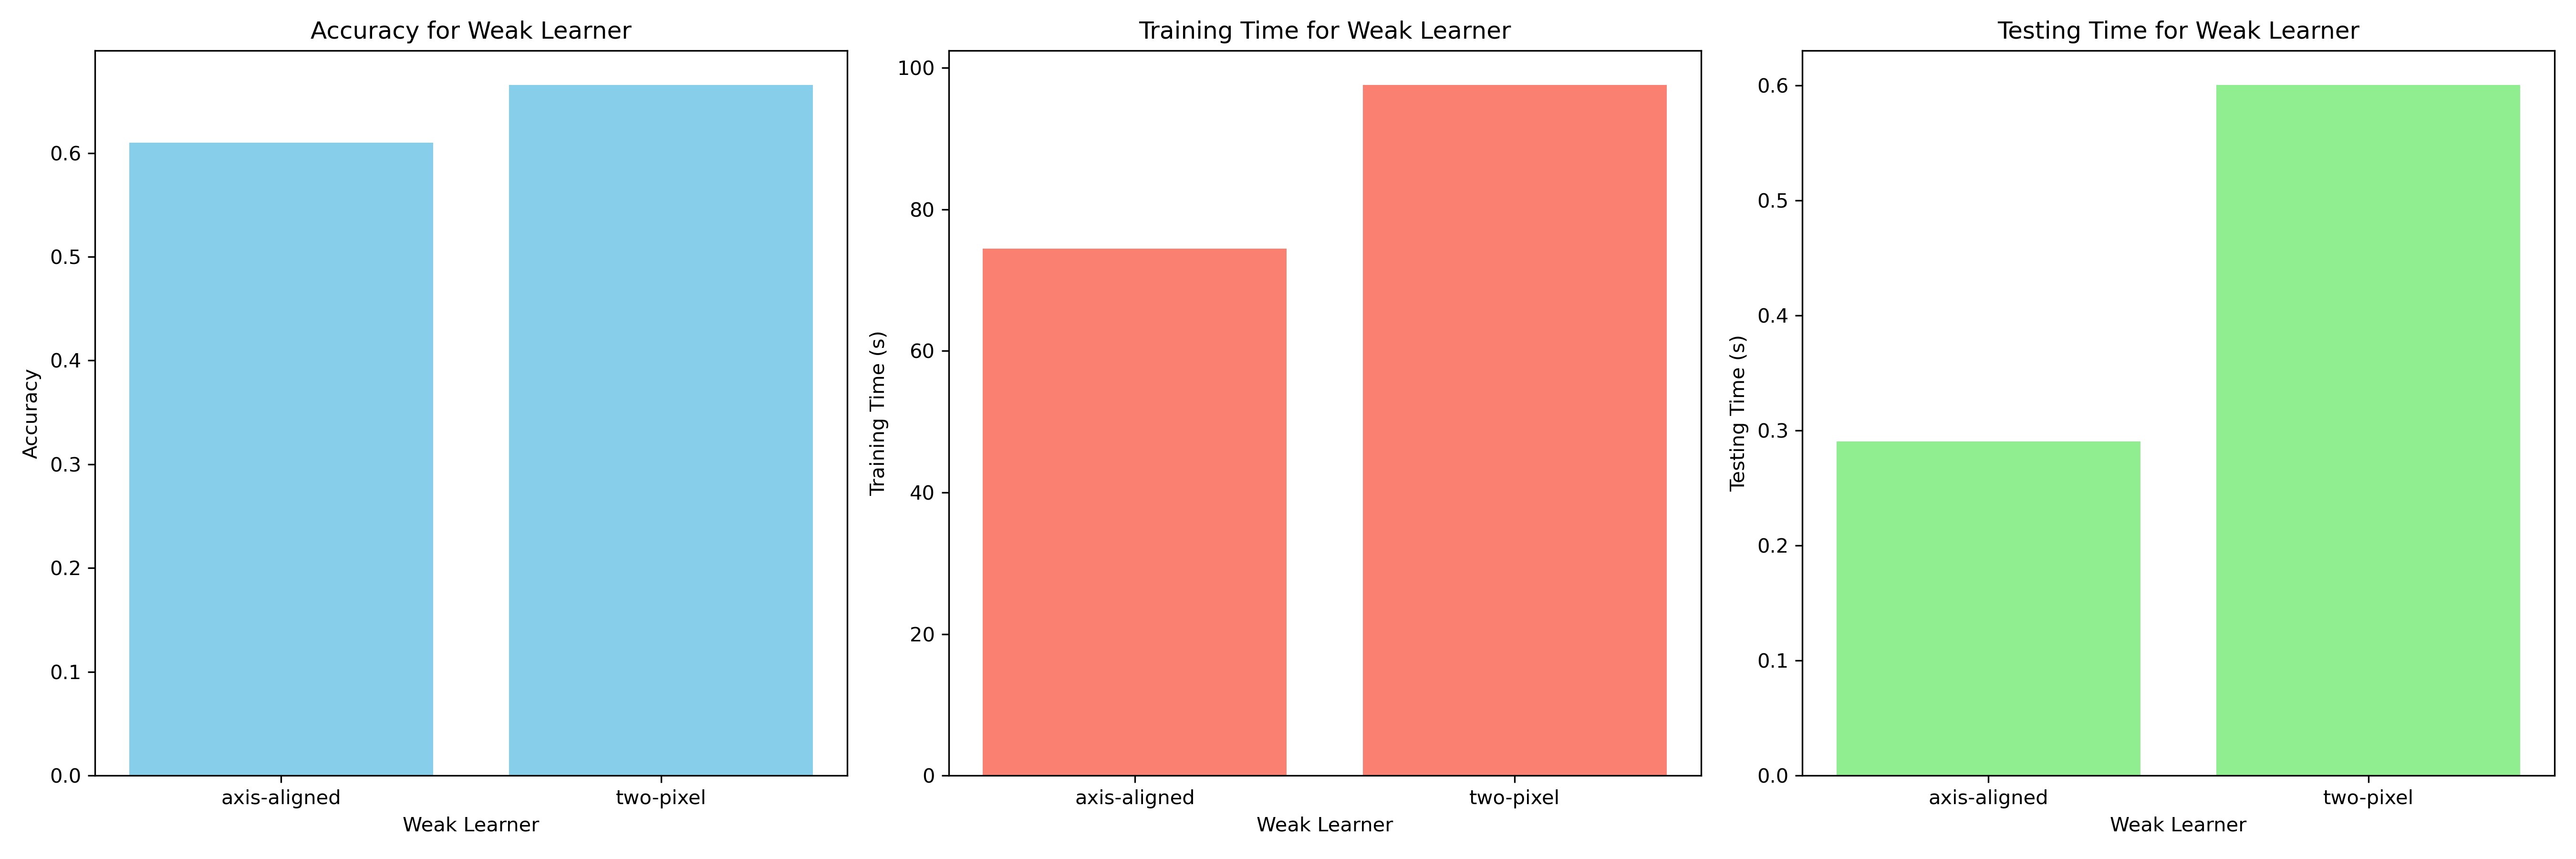
\includegraphics[width=0.8\linewidth]{image/q5-fig7.png}
	
	\caption{Axis-aligned vs Two-pixel test}
	\label{fig:q5-fig7}
\end{figure}


\subsection{Confusion matrix, Example success/failures, Information gain histogram}
The main results' confusion matrix, example success/failures, example node's histogram representing information gain along splitting are written in Appendix: \ref{subsec:Q5-1}, \ref{subsec:Q5-2}

\subsection{Comparision with PCA and PCA-LDA method}
Since parallel programming was not used our random forest, both the training and testing times are significantly large compared to the PCA and PCA-LDA methods. In addition, for PCA and PCA-LDA, the differences are further amplified due to Python NumPy’s parallelization for matrix operations and scikit-learn’s optimized KNN classification, which is well-tuned for handling multiple data points efficiently.
About the accuracy, because raw pixel values were used directly as inputs, the optimal accuracy of Q1 PCA is almost identical to random forest's result. Overall, the accuracy is much lower compared to the PCA-LDA method, indicating that in situations where the size of the training dataset is small ($N << D$), applying the random forest with no PCA is relatively less suitable. Additionally, similar to the PCA-LDA ensemble, as the number of base models (~tree) increases, there is a tendency for accuracy to improve, indicating that the 'ensemble models' is beneficial.


\onecolumn
\newpage
{\LARGE 
	\textbf{Appendix}\par}
\appendix
\section{Appendix}

\subsection{Q5: Test result's confusion matrix and success/failure cases }
\label{subsec:Q5-1}
The optimal parameters determined for the random forest through experiments are $N=250$, $D=8$, and $\text{splitnum}=10$. With this configuration, each real-time executable weak learner—axis-aligned and two-pixel tests—each was trained 10 times. The confusion matrix results below represent the best test accuracy among the 10 repetitive train results.

\begin{figure}[h]
	\centering
	\begin{subfigure}[t]{0.4\linewidth}
		\centering
		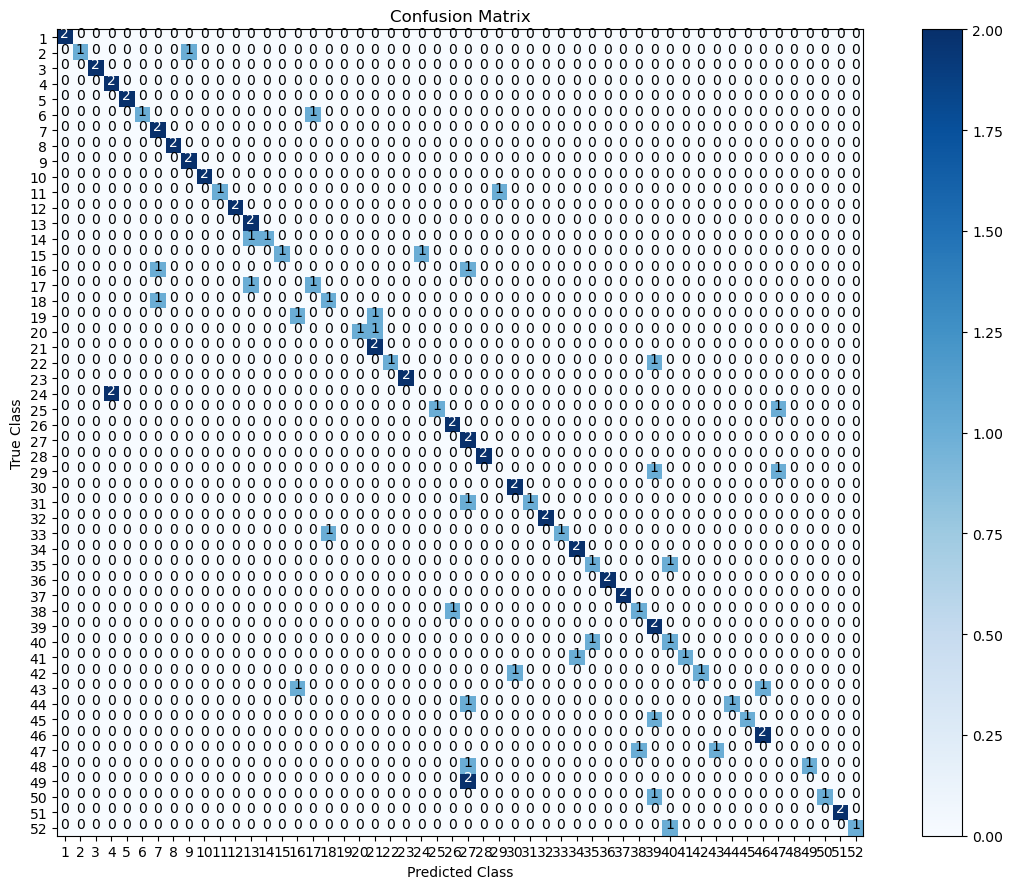
\includegraphics[width=\linewidth]{image/q5-fig6.png}
		\caption{Axis-aligned weak learner, test accuracy=0.644}
		\label{fig:q5-fig6}
	\end{subfigure}%
	\quad
	\begin{subfigure}[t]{0.4\linewidth}
		\centering
		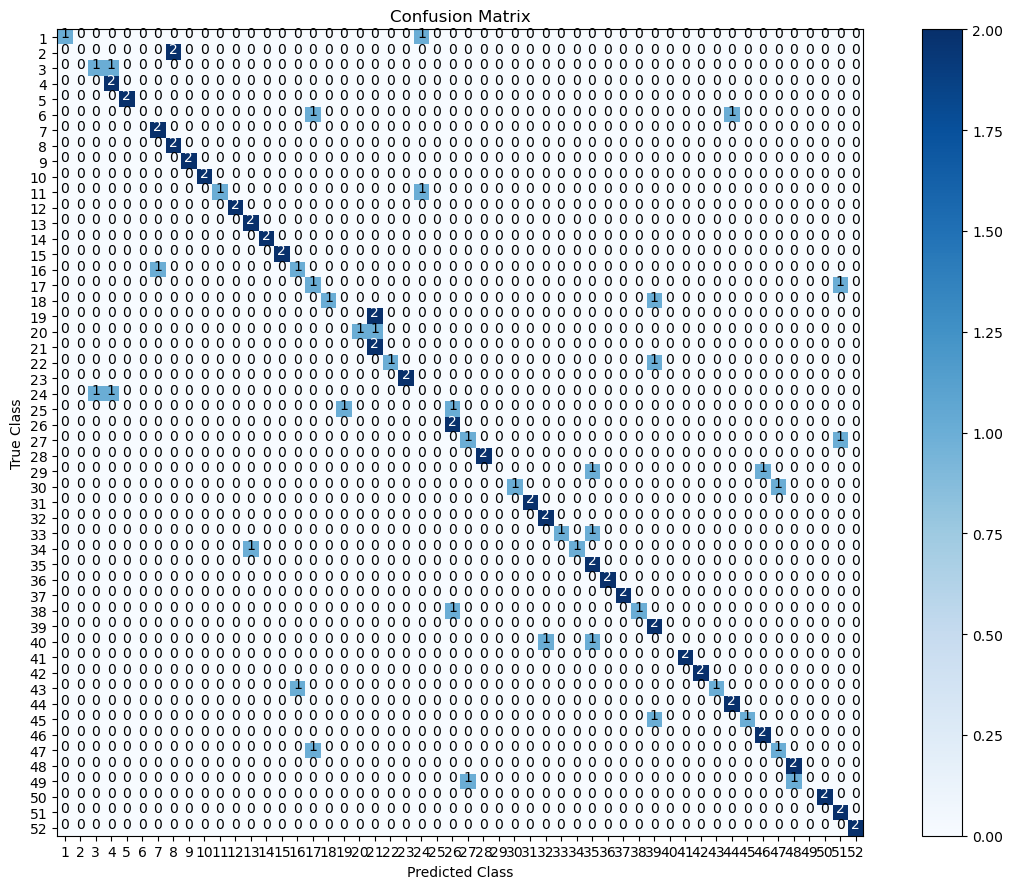
\includegraphics[width=\linewidth]{image/q5-fig8.png}
		\caption{Two-pixel test weak learner, test accuracy=0.692}
		\label{fig:q5-fig8}
	\end{subfigure}
	\caption{Confusion matrix of optimal cases ($N=250$, $D=8$, and $\text{splitnum}=10$)}
\end{figure}

Additionally, the example success and failure cases based on the confusion matrix results above are shown below. Compared to the success cases, the failure cases show a higher similarity between the failed image and the predicted class, meaning that our model is reasonable.
\begin{figure}
	\centering
	\begin{subfigure}{0.45\linewidth}
		\centering
		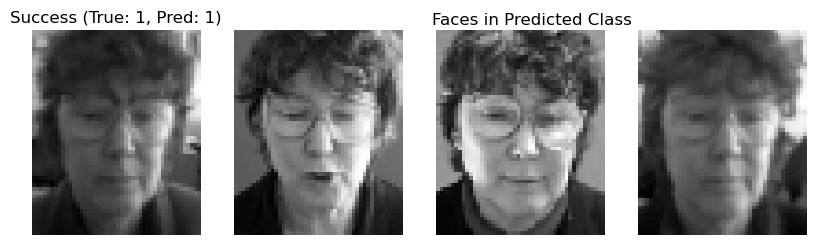
\includegraphics[width=\linewidth]{image/q5-app/q5-axis-succ1.png}
	\end{subfigure}%
	\quad
	\begin{subfigure}{0.45\linewidth}
		\centering
		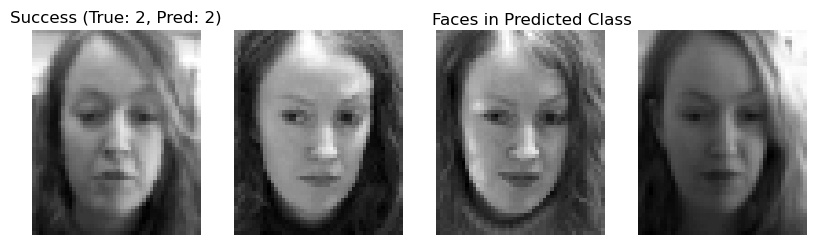
\includegraphics[width=\linewidth]{image/q5-app/q5-axis-succ2.png}
	\end{subfigure}
	\caption{Axis-aligned weak learner: Example success case}
\end{figure}
\begin{figure}
	\centering
	\begin{subfigure}[t]{0.45\linewidth}
		\centering
		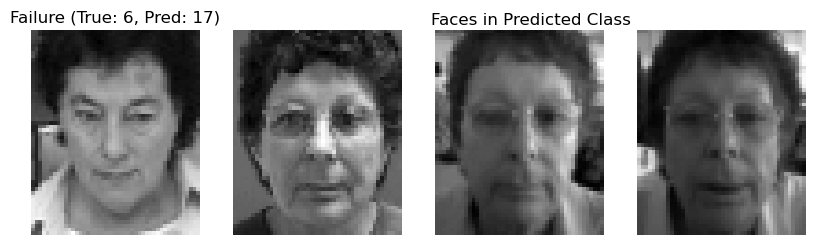
\includegraphics[width=\linewidth]{image/q5-app/q5-axis-fail1.png}
	\end{subfigure}%
	\quad
	\begin{subfigure}[t]{0.45\linewidth}
		\centering
		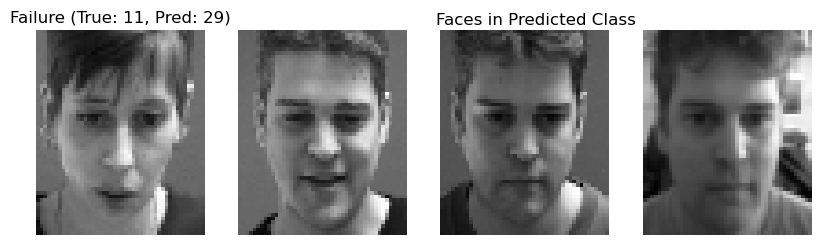
\includegraphics[width=\linewidth]{image/q5-app/q5-axis-fail2.png}
	\end{subfigure}
	\caption{Axis-aligned weak learner: Example failure case}
\end{figure}

\begin{figure}
	\centering
	\begin{subfigure}{0.45\linewidth}
		\centering
		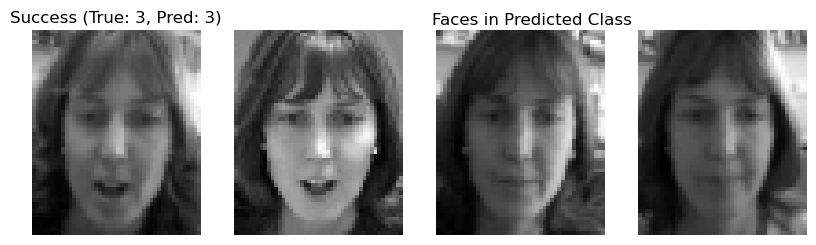
\includegraphics[width=\linewidth]{image/q5-app/q5-two-succ1.png}
	\end{subfigure}%
	\quad
	\begin{subfigure}{0.45\linewidth}
		\centering
		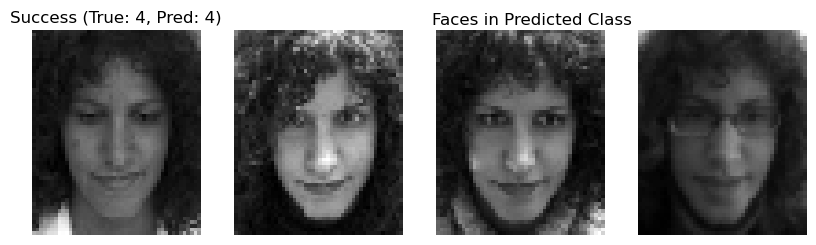
\includegraphics[width=\linewidth]{image/q5-app/q5-two-succ2.png}
	\end{subfigure}
	\caption{Two-pixel test weak learner: Example success case}
\end{figure}
\begin{figure}
	\centering
	\begin{subfigure}{0.45\linewidth}
		\centering
		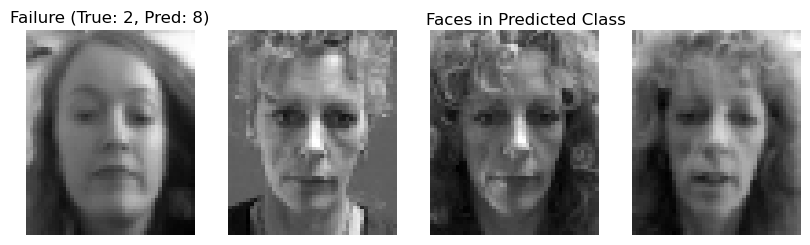
\includegraphics[width=\linewidth]{image/q5-app/q5-two-fail1.png}
	\end{subfigure}%
	\quad
	\begin{subfigure}{0.45\linewidth}
		\centering
		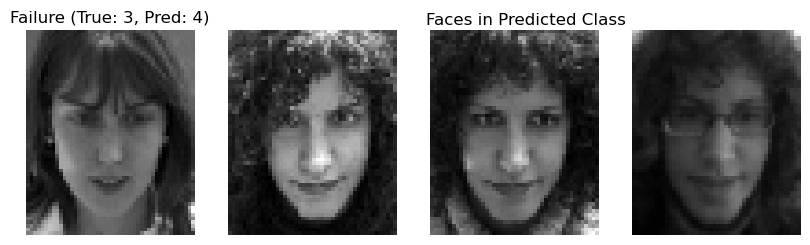
\includegraphics[width=\linewidth]{image/q5-app/q5-two-fail2.png}
	\end{subfigure}
	\caption{Two-pixel test weak learner: Example failure case}
\end{figure}

\subsection{Q5: Visualization of random forest's information gain process}
\label{subsec:Q5-2}

% WARNING: do not forget to delete the supplementary pages from your submission 
% \clearpage
\setcounter{page}{1}
\maketitlesupplementary


\section{Rationale}
\label{sec:rationale}
% 
Having the supplementary compiled together with the main paper means that:
% 
\begin{itemize}
\item The supplementary can back-reference sections of the main paper, for example, we can refer to \cref{sec:intro};
\item The main paper can forward reference sub-sections within the supplementary explicitly (e.g. referring to a particular experiment); 
\item When submitted to arXiv, the supplementary will already included at the end of the paper.
\end{itemize}
% 
To split the supplementary pages from the main paper, you can use \href{https://support.apple.com/en-ca/guide/preview/prvw11793/mac#:~:text=Delete%20a%20page%20from%20a,or%20choose%20Edit%20%3E%20Delete).}{Preview (on macOS)}, \href{https://www.adobe.com/acrobat/how-to/delete-pages-from-pdf.html#:~:text=Choose%20%E2%80%9CTools%E2%80%9D%20%3E%20%E2%80%9COrganize,or%20pages%20from%20the%20file.}{Adobe Acrobat} (on all OSs), as well as \href{https://superuser.com/questions/517986/is-it-possible-to-delete-some-pages-of-a-pdf-document}{command line tools}.

\end{document}
